%!TeX program = xelatex
%! BIB program = bibtex
\documentclass[zihao=-4]{ctexart}
\usepackage[normalem]{ulem}
\useunder{\uline}{\ul}{}
%********************导言区宏包引入********************
\usepackage{cite}
\usepackage{xeCJK}
\usepackage{amssymb}
\usepackage{amsmath}
\usepackage{listings} %代码
\usepackage{graphicx}
\usepackage{multicol} %回车换段
\usepackage{xcolor}
\usepackage{geometry} %页面设置
\usepackage{fontspec}
\usepackage{setspace}
\usepackage{times}
\usepackage{fancyhdr} %页眉页脚
\pagestyle{fancy}
\usepackage{float} %表格位置
\usepackage{titlesec} %设置
\usepackage{titletoc}
\usepackage{ctex}
\usepackage{gbt7714}    %控制参考文献格式为国标
\usepackage{multirow}
\usepackage{booktabs}   %表格相关
\usepackage{setspace}   %设置行距
\usepackage{caption} %caption
\usepackage{subcaption} %子图的caption
\usepackage{changepage} %左右缩进


\graphicspath{ {include_picture/} }
\let\algorithm\relax
\let\endalgorithm\relax
\usepackage[ruled,vlined]{algorithm2e}%[ruled,vlined]{
\usepackage{algpseudocode}
\renewcommand{\algorithmicrequire}{\textbf{Input:}} 
\renewcommand{\algorithmicensure}{\textbf{Output:}}
%\renewcommand\thepage{\zihao{-5} ~\arabic{page}~}%页码字号

%定义两个arg
\DeclareMathOperator*{\argmax}{arg\,max}
\DeclareMathOperator*{\argmin}{arg\,min}
\DeclareCaptionLabelSeparator{mysep}{\space\space}  %自定义caption格式
\captionsetup[figure]{labelfont=bf, labelsep=mysep, textfont=bf}   %图片caption格式
\captionsetup[table]{labelfont=bf, labelsep=mysep, textfont={bf}}   %表格caption格式
\bibliographystyle{gbt7714-numerical} %修改了title斜体内容

%********************导言区宏包引入********************
%********************第三方字体引入********************
%\setCJKmainfont[Path=fonts/,BoldFont=simhei.ttf,ItalicFont=simkai.ttf,SlantedFont=simfang.ttf]{simsun.ttc}
%中文字体涵盖黑体、宋体、楷体、仿宋
\setmainfont[Path=fonts/, 
BoldFont = times-new-roman-bold.ttf,
ItalicFont = times-new-roman-italic.ttf,
BoldItalicFont = times-new-roman-bold-italic.ttf
]{times-new-roman.ttf}
\setmonofont[Path=fonts/]{Courier New.ttf}
\setCJKfamilyfont{hwzs}[Path=fonts/]{STKzhongsong.ttf}%使用STZhogsong华文中宋字体
\newcommand{\zhongsong}{\CJKfamily{hwzs}}
\setCJKfamilyfont{hwxw}[Path=fonts/]{STKxinwei.ttf} % XSP 2023/3/3:
\newcommand{\xinwei}{\CJKfamily{hwxw}}              %  使用STZxinwei华文新魏字体.

%********************第三方字体引入********************


%********************中文字号设置********************
%\newcommand{\chuhao}{\fontsize{42pt}{\baselineskip}\selectfont}
\newcommand{\chuhao}{\fontsize{42pt}{0}}
\newcommand{\xiaochu}{\fontsize{36pt}{0}}
\newcommand{\yihao}{\fontsize{28pt}{0}}
\newcommand{\erhao}{\fontsize{21pt}{0}}
\newcommand{\xiaoer}{\fontsize{18pt}{0}}
\newcommand{\sanhao}{\fontsize{16pt}{0}}
\newcommand{\sihao}{\fontsize{14pt}{0}}
\newcommand{\xiaosi}{\fontsize{12pt}{0}}
\newcommand{\wuhao}{\fontsize{10.5pt}{0}}
\newcommand{\xiaowu}{\fontsize{9pt}{0}}
\newcommand{\liuhao}{\fontsize{8pt}{0}}
\newcommand{\qihao}{\fontsize{5.25pt}{0}}
%********************中文字号设置********************


%********************页边距设置********************
\geometry{left=3cm,right=2cm,top=2.5cm,bottom=2.5cm}
\geometry{a4paper} % xsp 2023/3/7: 调整纸张大小为A4
%********************页边距设置********************

%********************段间距设置********************
\newcommand{\setParDis}{\setlength {\parskip} {0pt} }
%请在每部分使用这个
%********************段间距设置********************

%********************

\begin{document}
%********************页眉页脚设置********************
\lhead{}%设置左页眉为空
\rhead{}%设置左页眉为空
\setlength{\headwidth}{\textwidth}% 2023/3/3 XSP: 页眉长度适应文本
%********************页眉页脚设置********************


%********************标题格式设置********************

%\setcounter{secnumdepth}{0}%该命令取消了章标题前数字label

\CTEXsetup[name={,、},number={\chinese{section}}]{section}
\CTEXsetup[name={(,)},number={\chinese{subsection}}]{subsection}
\CTEXsetup[name={,.},number={\arabic{subsubsection}}]{subsubsection}% 不加会导致目录格式错误
% 设置subsubsection等格式
% \titleformat{\section}[block]{\sanhao\bfseries\centering}{\chinese{section}、}{0pt}{}[]
% \titleformat{\subsection}[block]{\sihao\bfseries}{(\chinese{subsection})}{0pt}{}[]
% \titleformat{\subsubsection}[block]{\xiaosi\bfseries}{\arabic{subsubsection}、}{0pt}{}[]
\titleformat{\section}[block]{\sanhao\heiti\centering}{\chinese{section}、}{0pt}{}[]    % XSP 2023/3/3:
\titleformat{\subsection}[block]{\sihao\heiti}{(\chinese{subsection})}{0pt}{}[]       %   将正文标题字体由加粗
\titleformat{\subsubsection}[block]{\xiaosi\heiti}{\arabic{subsubsection}.}{0pt}{}[]   % 修改为黑体。
\titlespacing{\section}{0pt}{25pt}{12pt}
\titlespacing{\subsection}{0pt}{7pt}{7pt}
\titlespacing{\subsubsection}{0pt}{5pt}{4pt}

\titlecontents{section}[1.6em]{\addvspace{2pt}\filright}
{\contentspush{\thecontentslabel\hspace{0.8em}}}
{}{\titlerule*[8pt]{.}\contentspage}

\titlecontents{subsection}[3.2em]{\addvspace{2pt}\filright}
{\contentspush{\thecontentslabel\hspace{0.8em}}}
{}{\titlerule*[8pt]{.}\contentspage}

\titlecontents{subsubsection}[6.4em]{\addvspace{2pt}\filright}
{\contentspush{\thecontentslabel\hspace{0.8em}}}
{}{\titlerule*[8pt]{.}\contentspage}
%********************标题格式设置********************

%\setcounter{section}{-3}  %标题计数器
%\stepcounter{section}

%*******************行间距段前段后*******************
\linespread{1.8}
%行间距为实际行间距乘以1.2,如此处实际为1.5倍行距
\setlength{\parskip}{0.5\baselineskip}
%*******************行间距段前段后*******************



%********************封面部分********************
%
%     论文题目:应准确、鲜明、简洁,能概括整个论文中最主要和最重要的内容。
% 题目不超过20个中文字,若语意未尽,可用副标题补充说明。副标题应处于从属
% 地位,一般可在题目的下一行用破折号“——”引出。论文题目应避免使用不常用缩
% 略词、首字母缩写字、字符、代号和公式等。
%
\leftline{
\includegraphics[scale=1]{include_picture/xiaohui.png}} % XSP 2023/3/3: 取消校徽段首缩进
%格式控制部分
% \par \  
% \par \
% \par \
\vspace{32pt}
\begin{center}

\includegraphics[height=2.25cm, width=12.78cm, scale=1]{include_picture/xiaoming.png}
\end{center}
%格式控制部分
\vspace{12pt}

\begin{spacing}{3}
    % \erhao
    \begin{center}
        \zhongsong\erhao{第三十三届“冯如杯”竞赛主赛道项目论文模板} %黑体这样调用,其余字体同理
        
        % \zhongsong{“冯如杯”竞赛主赛道项目是什么}
    \end{center}
    \rightline{\xinwei\sanhao{——基于 Latex 的论文模板}} % XSP 2023/3/3: 副标题二号华文新魏居右
\end{spacing}
%格式控制部分
% \par \ 
% \par \
\par \ 
\par \
\par \ 
\par \
% \begin{center}
%     \sihao
%     \textbf{学院:计算机学院}
%     \par \ 
%     \textbf{本模板原作者:Someday}
% \end{center}

%格式控制部分
\par \ 
\begin{center}
\sanhao
\centerline{\heiti{}}%封面年月去掉
\end{center}

\pagenumbering{gobble} %封面无页码
%\thispagestyle{empty}


\renewcommand{\headrulewidth}{0pt}%没有页眉装饰线
\clearpage
\pagenumbering{roman} %摘要目录页小写罗马

\xiaosi
\section*{摘要}
\begin{spacing}{1.5}
  \setParDis %设置段间距为 0
  本Latex模板是北京航空航天大学大学第三十三届“冯如杯”竞赛主赛道论文模板, 由北京航空航天大学校团委
基于GitHub用户\textbf{\textit{Somedaywilldo}}与\textbf{\textit{cpfy}}的成果迭代
开发而来。在此由衷感谢所有开发者对本模板的贡献与对“冯如杯”竞赛的大力支持。

摘要内容包括:“摘要”字样,摘要正文,关键词。在摘要的最下方另起一行,用显著的字符注明文本的关键词。

摘要是论文内容的简短陈述,应体现论文工作的核心思想。摘要一般约500字。摘要内容应涉及本项科研工作的目的和意义、研究思想和方法、研究成果和结论。

关键词是为用户查找文献,从文中选取出来用来揭示全文主题内容的一组词语或术语,应尽量采用词表中的规范词(参照相应的技术术语标准)。关键词一般为3到8个,按词条的外延层次排列。关键词之间用逗号分开,最后一个关键词后不打标点符号。

\end{spacing}
    
\textbf{关键词:}关键词1,关键词2,关键词3,关键词4,关键词5

\newpage
\section*{\textbf{Abstract}} % XSP 2023/3/8: Abstract 加粗
\begin{spacing}{1.5}
\begin{adjustwidth}{0.42cm}{0.42cm}
  \setParDis %设置段间距为 0

\qquad This Latex template for the 33rd Fengru Cup Competition of 
Beihang University, is developed by Communist Youth League Committee of BUAA 
iteratively based on the contribution of GitHub 
users \textbf{\textit{Somedaywilldo}} and \textbf{\textit{cpfy}}. 
Here, we would like to thank all the developers for their 
contributions to this template and for their support of the Fengru Cup Competition.

The abstract includes: the word "Abstract", the body of the abstract, and the keywords. On a separate line at the bottom of the abstract, indicate the key words of the text in prominent characters.

The abstract is a short statement of the content of the paper and should reflect the core ideas of the paper work. The abstract is usually about 500 words. The abstract should cover the purpose and significance of this scientific work, research ideas and methods, research results and conclusions.

Keywords are a set of words or terms selected from the text to reveal the subject content of the whole text for the user to find the literature, and the standardized words in the word list (refer to the corresponding technical terminology standards) should be used as much as possible. The keywords are usually 3 to 8, arranged according to the level of extensibility of the words. The keywords are separated by commas, and no punctuation marks are used after the last keyword.

\textbf{Keywords: Keywords 1, Keywords 2, Keywords 3, Keywords 5, Keywords 6}
\end{adjustwidth}
\end{spacing}



%********************摘要部分********************


%********************目录部分********************
\clearpage
\tableofcontents
\clearpage
%********************目录部分********************



\renewcommand{\headrulewidth}{0.4pt} %恢复页眉装饰线

%********************正文页眉部分********************
%\lhead{} 
\chead{\xiaowu 北京航空航天大学第三十三届“冯如杯”竞赛主赛道参赛作品} %设置居中页眉
%********************正文页眉部分********************

\pagenumbering{arabic} %正文页码从1开始,用阿拉伯数字
\setcounter{page}{1} 




%********************作品概述********************
\section{作品概述}
本章首先介绍基于位置信息隐私保护的研究背景和研究意义,接着介绍国内外相关领域的研究现状,然后引出本文研究的主要内容,最后给出本文各章节的内容安排。

\subsection{研究背景与研究意义}
近年来,移动用户数量迅猛增长,越来越多的用户选择使用移动设备来满足他们的日常活动需求,而不是依靠电脑。
\cite{czh_1.1}在此背景下,基于位置的服务(Location Based Services, LBS)成为了一种趋势。基于位置的服务是指服务提供商根据用户提交的位置信息,返还给用户对应的基于位置信息的相应服务。
比如大多数现代服务系统都会要求用户发送他们的位置信息,以提供更具适应性、符合用户实际需求和偏好的服务,例如关于天气、交通的警报服务或者提供出行的最佳路线。\cite{czh_1.2}
\par
在用户提交的位置信息中,最常用、便于服务提供商进行处理的位置信息是用户直接的地理位置信息,这也和用户个人隐私安全有着密切关系。但是,当移动应用频繁询问用户所在位置信息时,用户的位置信息面临着暴露的风险,甚至用户的其他隐私也不再安全。比如不可信的服务提供商可以利用用户的位置信息和上传时间,结合大数据分析手段绘制出用户的时间活动轨迹和活动热点图,进一步分析出用户的行为习惯、具体身份、社交信息等敏感隐私。在更极端的情况下,服务提供商还可以分析出用户的隐私画像,对匿名用户进行去匿名化,严重威胁用户隐私安全。
\par
但是事实上相当多的移动应用都会询问用户的位置信息,这也带来了泄露位置信息、侵犯隐私的隐患。
以Google应用市场为例,根据2017年的统计数据,在最受欢迎的2800个移动应用(aplication,简称app)中,4成以上的app要求用户提供访问位置信息的权限,其中包括在后台可以直接访问位置的app,\cite{czh_1.3}这在当时引起了用户群体一定的抗议。
然而遗憾的是,当前大多数服务提供商对位置信息的保护力度远远不够。
用户通常只能简单选择“是”或“否”给予服务提供商具体位置,而不能选择被上传的用户位置的精度,也没有对位置数据后续使用情况的追溯权限。
服务提供商以使用用户地理位置提供精准服务的名义,将可能侵犯隐私的数据条款隐藏在繁杂的用户条款中,将用户摆在了无法反制的弱势地位上。
现行的大多数隐私保护方案都基于通信渠道的安全性和授权,在获取位置信息后,服务提供方并没有对这些敏感信息给予应有的保护,
\cite{czh_1.4}在这样的环境下,如何保护位置信息的隐私安全成为了一个新的问题。
\par
需要注意的是,在保护位置信息隐私安全的同时,我们还应该保证位置信息的真实性以及用户获得的服务质量。
如果忽略了位置信息的真实性,那么在一些特殊情景下,用户可能会向系统提供错误的位置信息来达成某些目的。
比如攻击者可以向系统发送虚假的位置信息,以寻求系统的漏洞;或者用户可以在发生交通事故肇事逃逸后提交错误的位置信息,以逃避追责\cite{czh_1.5}。
而保护隐私后的服务质量也同样需要保障。当前保护位置隐私信息的一种重要方式是模糊用户的实际位置,将用户位置信息隐藏在虚假的位置或者一个模糊的范围中。
这样固然对位置隐私起到一定的保护作用,却可能降低用户获得的服务质量,影响用户的服务体验。
这两个需求也对现有位置隐私保护方案提出了更高的要求。
\par
而现有的大多数位置隐私保护方案要么在在保护用户位置信息安全上存在漏洞,要么在满足上述两种需求上存在进一步提高的空间。并且用户基本只能选择同意授权获取位置权限或者拒绝,而难以在授权的同时控制暴露的位置信息的精度。因而服务提供商可以借提供服务的名义收集用户位置信息,这也使得用户处在一个难以保护自己隐私的弱势地位上。
在这样的背景下,如果可以探索出一种新的位置隐私保护方案,这将为保护用户位置信息安全提供极大助力,并进一步促进隐私保护领域相关技术的发展。
同时,如果将新的方案技术移植应用到其他领域,那将会为各行业的数据信息安全提供更可靠的保障。


\subsection{研究现状}
随着移动设备用户数量逐年增加和服务精细化成为一种趋势,LBS开始广泛应用在日常生活中。而在用户享受服务的同时,用户的位置信息可能会被服务提供商或攻击者采集进而造成隐私泄露。为了解决用户位置隐私的安全,国内外研究人员对位置信息保护模型进行了广泛的研究,迄今为止已经初步形成了若干成熟的位置隐私保护模型和相关的保护技术。本节将对其中比较成熟、应用比较广泛的位置隐私保护系统结构以及相关技术技术进行介绍。

\subsubsection{位置隐私保护系统结构}
现行的基于位置的隐私保护系统主要有3种结构,分别是集中式结构、分布式结构以及混合式结构。这三种结构各有优缺点,分别适用不同的应用场景。
\par 
\textbf{(1)集中式结构}
\par 
集中式结构在客户端和服务提供商之间加入位置匿名服务器,帮助用户进行位置匿名处理,并帮助用户从模糊的服务集合中筛选出用户实际需要的服务。\cite{czh_6.1}引入位置匿名服务器后,移动用户端的计算、存储负担大为减小,一些复杂的算法、功能也有了实现的可能。但是引入第三方服务器也带来了一些问题。一旦服务器受到攻击并泄露信息,或者服务器不再可信,用户的位置隐私将被泄露。
\par 
\textbf{(2)分布式结构}
\par 
鉴于集中结构位置匿名服务器带来的安全问题和性能瓶颈问题,分布式结构去除了位置匿名服务器,并通过多台移动设备之间的协作来实现位置匿名效果。用户发起查询请求后,多个移动设备相互协作形成一个匿名区域,从而将用户真实的位置信息隐藏在这个区域中。这种结构与集中式结构相比无疑更加安全,但是却也对用户移动设备的计算能力提出了一定的要求。
\par 
\textbf{(3)混合结构}
\par 
基于集中式结构和分布式结构的优点,混合结构同时使用了两种结构。用户既可以通过位置匿名服务器完成匿名,也可以通过多台移动设备协助来形成一个匿名区域。虽然混合式结构集中了之前两种结构的优点,但是这种结构也存在一定的缺点。在构建和维持混合式系统结构时需要不断设置、调整参数\cite{czh_6.2},以决定系统在不同条件下选择哪种方式来完成用户和服务提供商之间的通信,这也束缚了混合结构的进一步发展。

\iffalse
\textbf{待删改}
现行的基于位置的隐私保护系统主要有3种结构:集中式结构、分布式结构以及混合式结构。国内外研究人员在这3种结构的基础上迭代出了很多高效、具有广泛适用性的位置信息隐私保护算法。本节将简要介绍这3种系统结构,并概括出各种结构的优缺点。

\subsubsection{集中式结构}
集中式结构在基本已被淘汰的独立结构(仅由用户和服务提供方组成客户端/服务器结构$^{[2.1]}$)的基础上进行改进,在客户端和服务器之间加入位置匿名服务器,以分担客户端的计算、存储开销。集中式结构的示意图见图\ref{集中式结构}。

\begin{figure}[H] %H为当前位置,!htb为忽略美学标准,htbp为浮动图形
	\centering %图片居中
	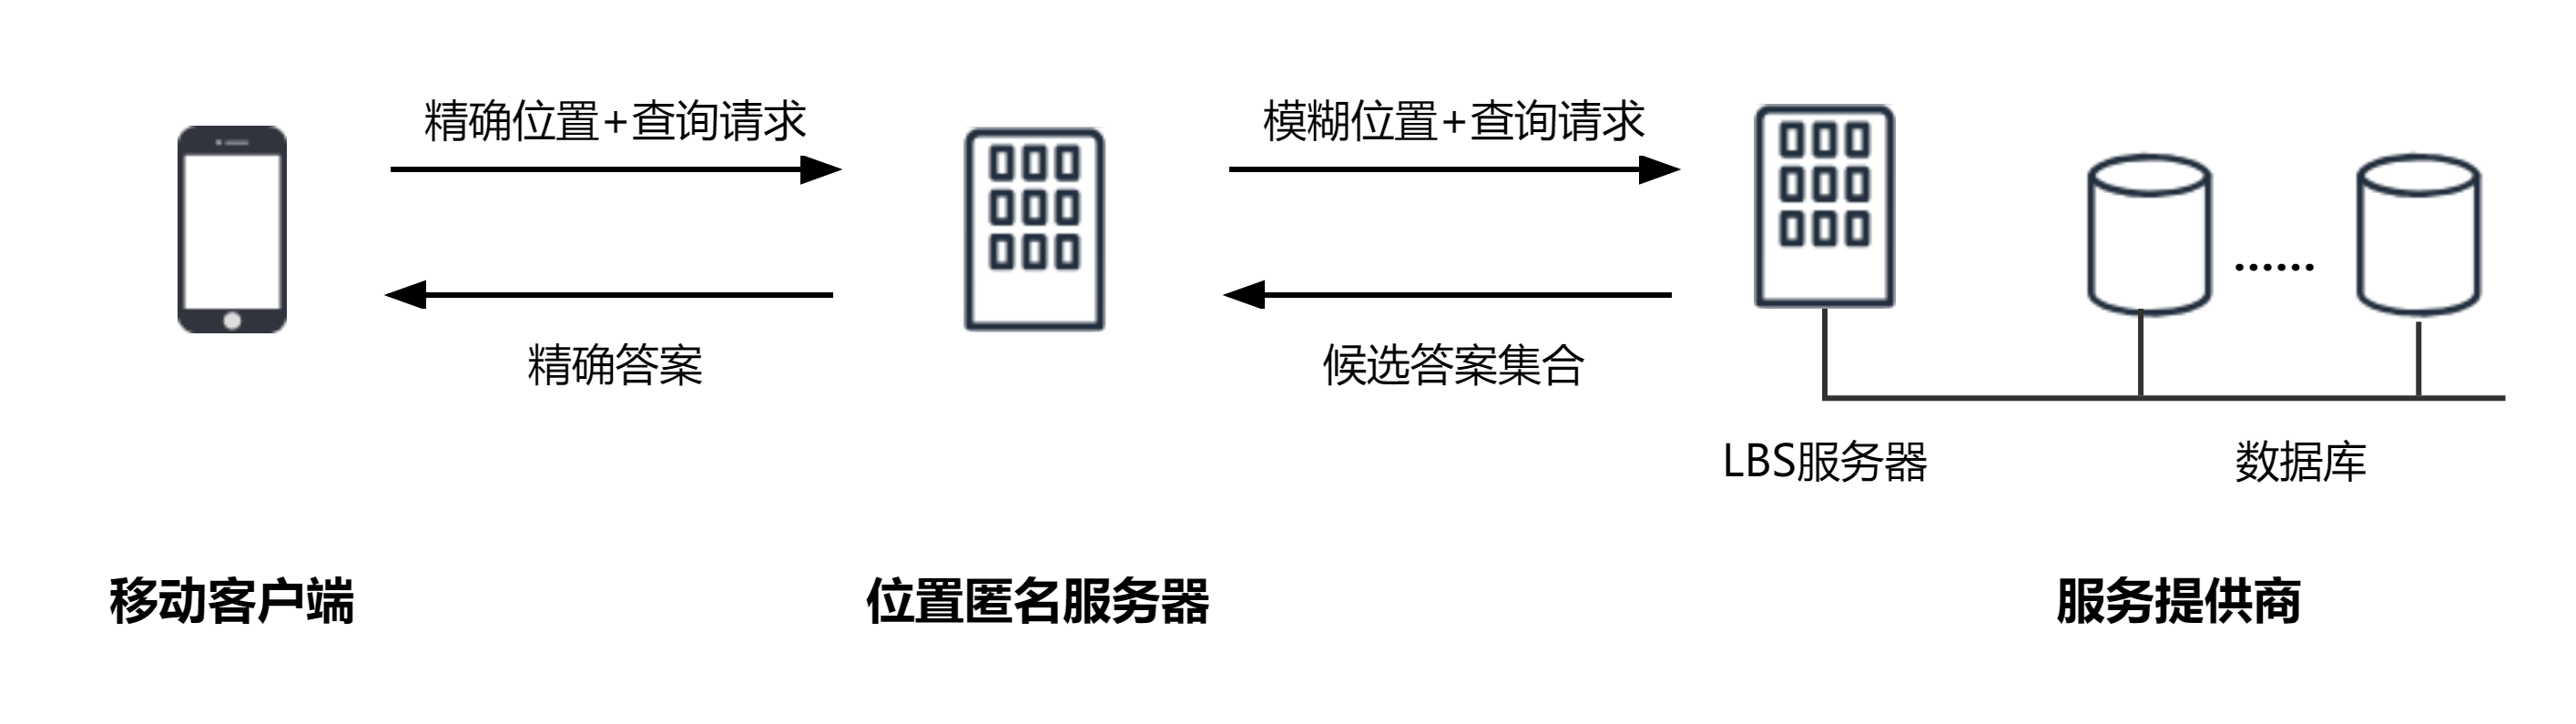
\includegraphics[width=0.8\textwidth]{./include_picture/集中式结构(绪论-研究现状)} %插入图片,[]中设置图片大小,{}中是图片文件名
	\caption{集中式结构系统示意图} %最终文档中希望显示的图片标题
	\label{集中式结构} %用于文内引用的标签
\end{figure}

在集中式结构的位置隐私保护系统中,用户发起查询请求后,由位置匿名服务器对用户的精确位置进行匿名处理。服务提供商收到位置匿名服务器提交的查询请求后,根据接受到的位置返回用户可能需要的答案集合,称为候选答案集合。位置匿名服务器接收到答案集合后,根据用户的精确位置进行筛选求精操作,最终把精确答案返还给用户。$^{[czh\_2.2]}$
\par
引入位置匿名服务器为系统性能带来了显著的提高。一方面,位置匿名服务器承担了位置匿名处理、候选答案求精的任务,从而减轻了用户端的负担,使得用户端的设计可以更为轻量。另一方面,引入位置匿名服务器后,原本一些在移动客户端上难以实现的复杂算法、功能也有了实现的可能,系统功能更加强大。
\par
当然,位置匿名服务器本身也有一些缺点。随着系统的使用,服务器中存储的用户位置数据会逐渐积累。如果没有对服务器存储的数据进行处理,一旦服务器被攻击、或者服务器不再可信,这将会严重损害用户的位置信息隐私安全。此外,当系统用户频繁请求服务时,服务器自身的性能也可能成为限制系统性能的瓶颈。$^{[czh\_2.1]}$


\subsubsection{分布式结构}
鉴于集中结构位置匿名服务器带来的安全问题和性能瓶颈问题,分布式结构去除了位置匿名服务器的存在,而是通过多台移动设备之间的协作来实现位置匿名效果。分布式系统结构示意图见图\ref{分布式结构}。
\begin{figure}[H] %H为当前位置,!htb为忽略美学标准,htbp为浮动图形
	\centering %图片居中
	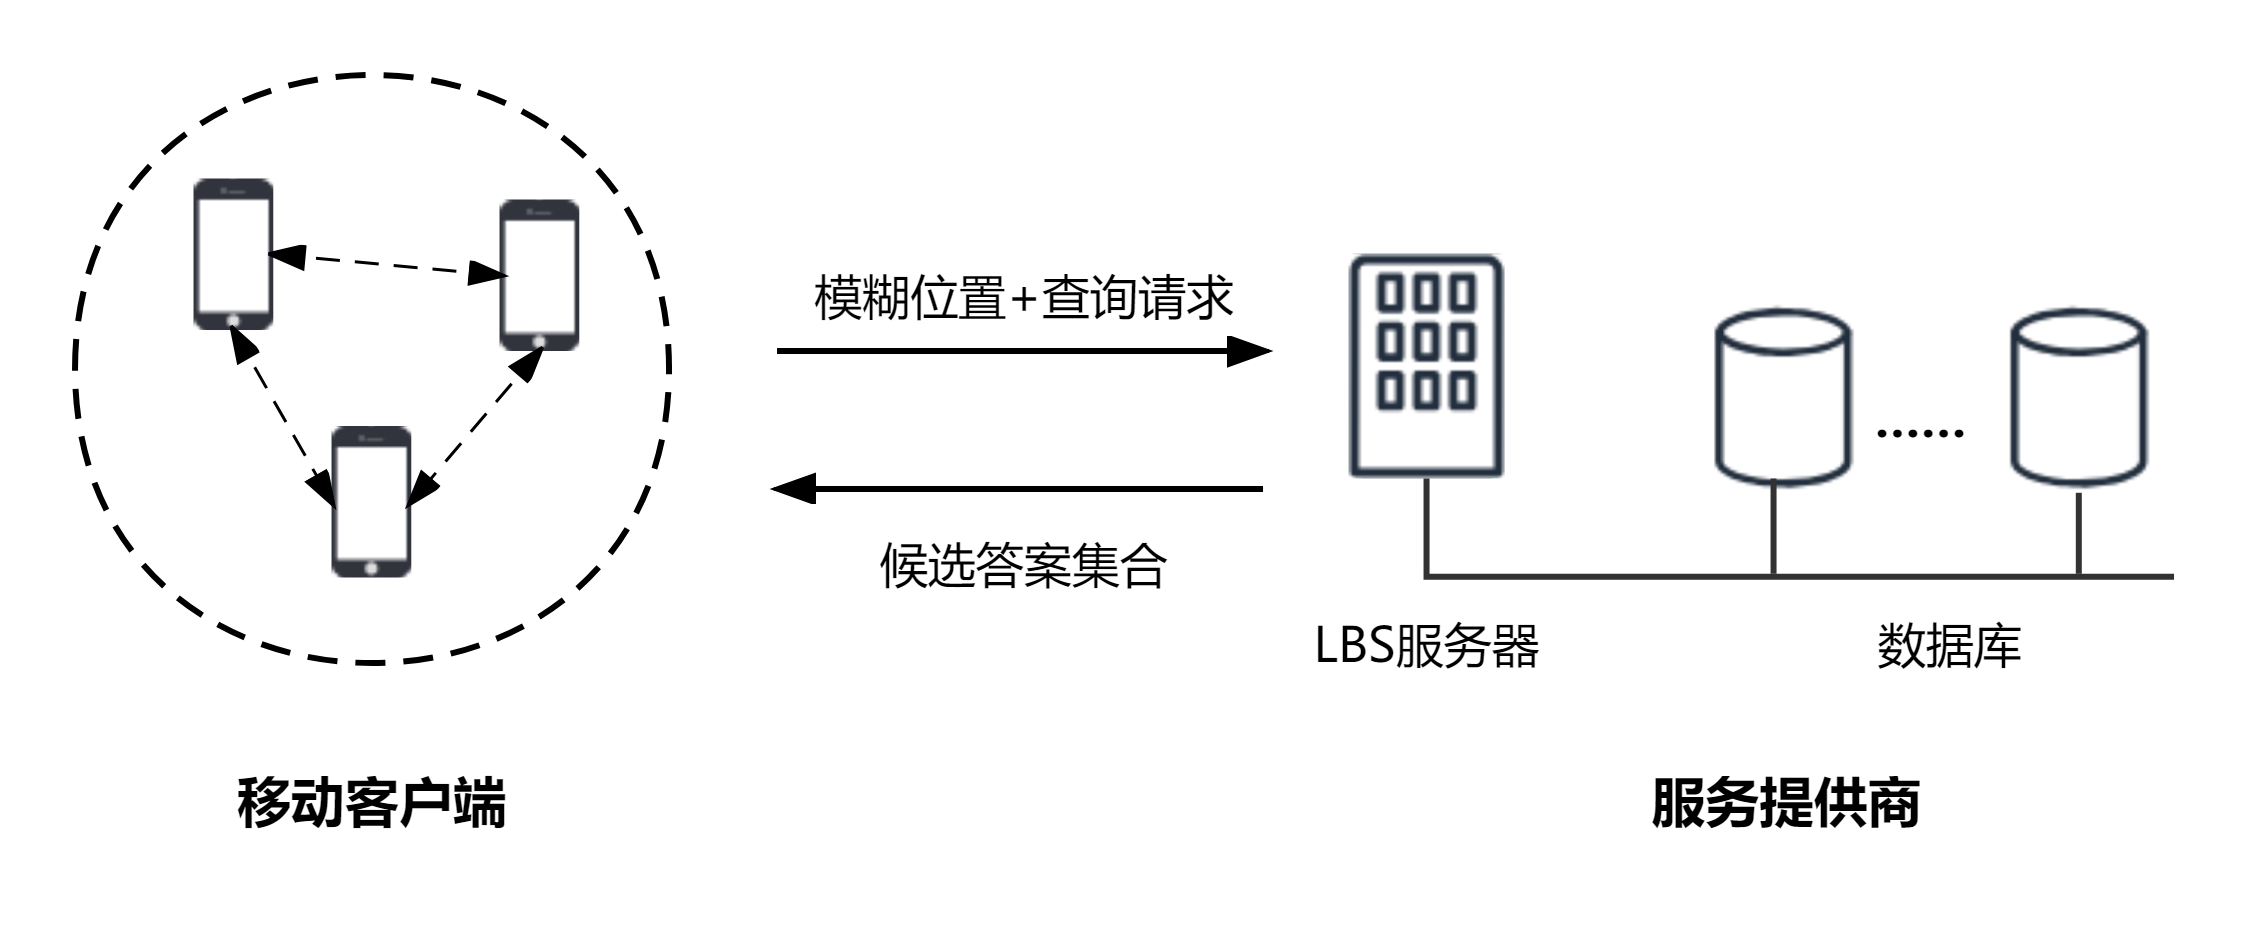
\includegraphics[width=0.8\textwidth]{./include_picture/分布式点对点结构(绪论-研究现状)} %插入图片,[]中设置图片大小,{}中是图片文件名
	\caption{分布式结构系统示意图} %最终文档中希望显示的图片标题
	\label{分布式结构} %用于文内引用的标签
\end{figure}

在分布式结构系统中,用户发起查询请求后,一定区域内的多台移动设备相互协作并进行一定的通信,形成一个匿名区域。服务提供商根据接收到的区域返回相应的候选答案集合,用户接受到答案集合后进行筛选和求取精确答案的操作。
\par
和集中式结构相比,分布式结构的系统进一步降低了用户位置信息泄露的隐患。但分布式结构也对用户移动设备的计算能力提出了一定的要求,以便进行协作匿名。这也限制了分布式结构系统的发展。$^{[czh\_2.1]}$

\subsubsection{混合结构}
考虑到集中式结构系统的计算能力以及分布式结构系统的信息保密性,部分系统融合了上述两种结构,形成了兼具上述优点的新的系统结构——混合结构。混合结构的系统示意图见图\ref{混合结构}。
\begin{figure}[H] %H为当前位置,!htb为忽略美学标准,htbp为浮动图形
	\centering %图片居中
	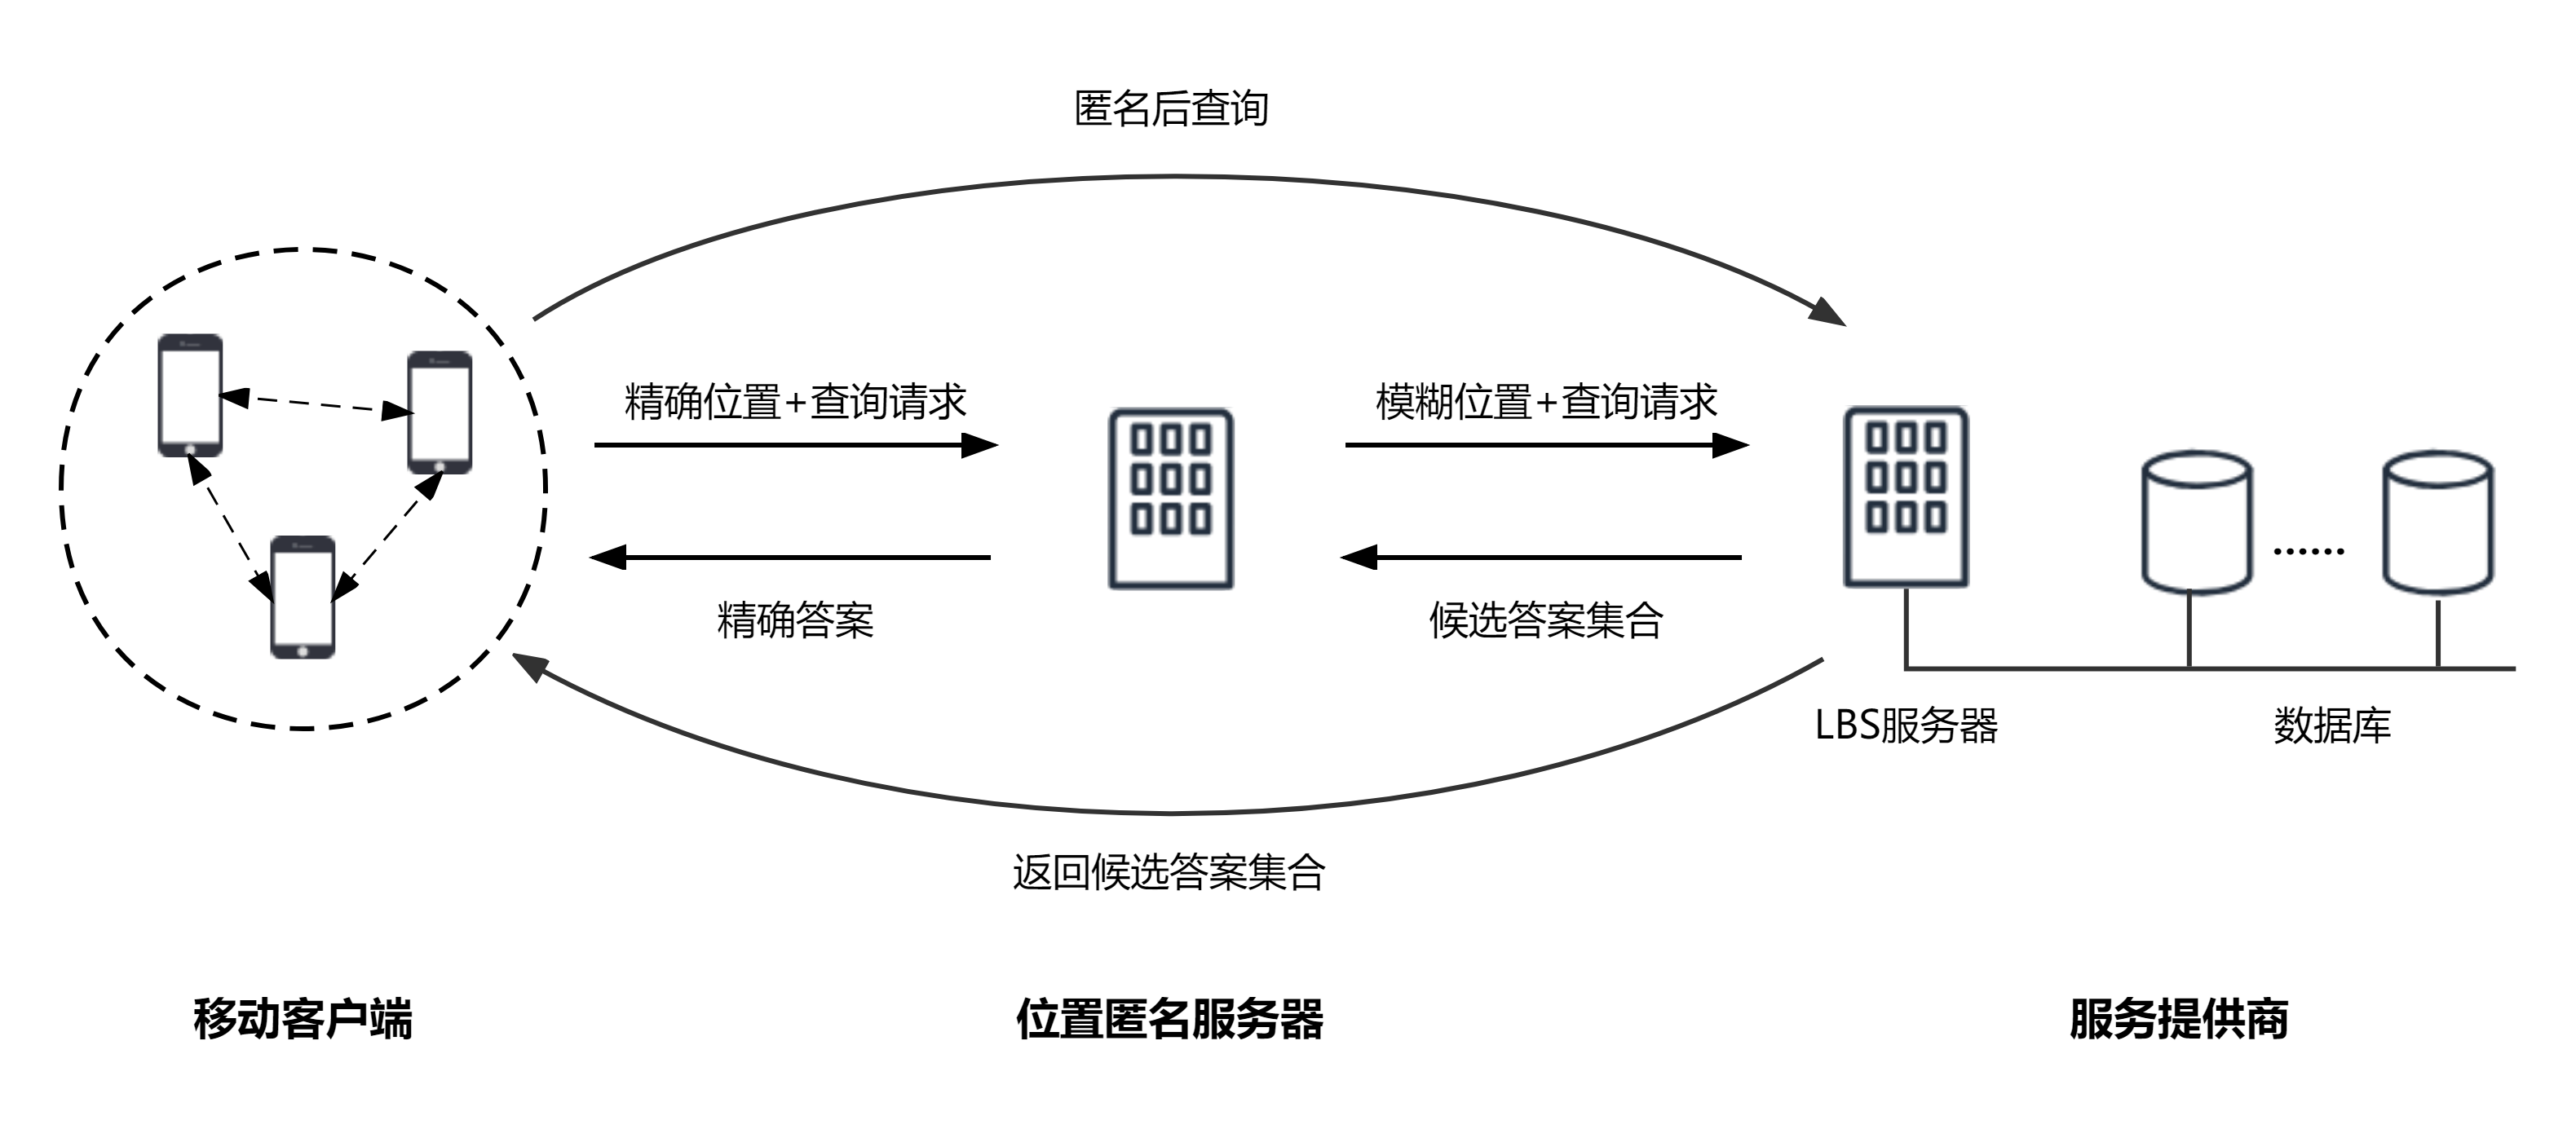
\includegraphics[width=0.8\textwidth]{./include_picture/混合结构(绪论-研究现状)} %插入图片,[]中设置图片大小,{}中是图片文件名
	\caption{混合结构系统示意图} %最终文档中希望显示的图片标题
	\label{混合结构} %用于文内引用的标签
\end{figure}

在混合结构系统中,用户发起查询请求后,系统可以选择让用户通过位置匿名服务器进行匿名查询,也可以联合多台移动设备,通过分布式的方式直接和LBS服务器取得联系,这将取决与系统中发起查询请求的用户数量。
\par
值得一提的是,虽然混合结构吸收了先前两种结构的优点,使它看上去更为灵活。但实际上,在构建和维持混合结构时需要不断设置、调整系统参数,以决定系统什么时候通过哪种方式和LBS服务器建立联系。这也束缚了混合结构的进一步发展$^{[czh\_2.3]}$。
\par \par 
在上面的3个小节中,我们介绍了现行基于位置隐私保护系统的3种主要结构,它们各自的优缺点可以概括为表\ref{3种结构对比}。
\fi 

\begin{table}[H]
	\caption{位置隐私保护系统3种结构对比}
	\centering
	\label{3种结构对比}
	\begin{tabular}{ccc}
		\hline  
		\makebox[0.1\textwidth][c]{结构名称} & \makebox[0.4\textwidth][c]{优点} & \makebox[0.4\textwidth][c]{缺点}  \\ 
		\hline  
		集中式结构	&	计算、存储性能提高	&	有泄露隐私的风险\\
		分布式结构	&	提高安全性		   &	对移动设备性能要求较高\\
		混合结构	 &	兼具安全性和性能	 & 		系统参数限制了应用\\
		\hline
	\end{tabular} 
\end{table} 

\iffalse 
在以上3中位置隐私保护结构的基础上,国内外学者研发出了多种位置隐私保护技术。其中比较著名的有将用户位置信息隐藏在虚拟位置中的\textbf{K-匿名技术}$^{[czh\_2.4]}$,在真实位置信息中添加虚假信息的\textbf{虚假位置技术}$^{[czh\_2.5]}$等等。由于本文主要在系统结构进行创新,这些技术不再一一说明。
\fi


\subsubsection{位置隐私保护技术}
位置隐私保护方法主要从位置数据加密、匿名位置区域和差分隐私等方面考虑,其中匿名位置区域、差分隐私两个方向近年来不断发展,应用前景相对可观,本部分也将着重介绍这两个方向的研究进展。
\par 
\textbf{(1)位置数据加密}
\par 
位置数据加密方法通过加密算法对位置信息进行加密,从而达到保护位置隐私的效果。如Zhu等人基于加密算法提出一个隐私保护框架,将LBS外包到云中,并允许用户动态控制精度,从而在服务和隐私之间进行权衡。\cite{czh_6.3}
\par 
\textbf{(2)匿名位置区域}
\par 
在基于匿名位置区域的位置隐私保护技术中,比较成熟的是K-匿名技术。基于用虚假位置代替用户真实位置的想法,Pierangela等首次提出K-匿名隐私保护技术,通过泛化的方式保护数据隐私。\cite{czh_6.4}在此基础上,Gruteser等\cite{czh_6.5}提出一种假位置数据隐私保护模型,将产生的几个虚假位置混淆在用户真实位置中,从而达到匿名效果。K-匿名隐私保护技术和当前分布式系统结构有较高的相容性,使用时也比较灵活,但是匿名效果依赖于K值的选取。K值太小时匿名效果难以保持,但是当K值较大时,系统将会承担很多不必要的计算开销。另外,K-匿名隐私保护技术也依赖于分布式系统结构,用户在对位置信息进行匿名化时计算开销较大。
\par 
\textbf{(3)差分隐私}
\par 
差分隐私有数学基础作为支撑,可被公式证明可以抵挡攻击者的背景攻击,具有可靠的安全下限。在2006年,Cynthia Dwork等\cite{czh_6.6}基于不可区分性运用拉普拉斯分布,首次提出差分隐私。在此基础上,Frank等\cite{czh_6.7}提出差分隐私指数机制,并基于各种差分隐私机制将其运用到数据查询、数据挖掘等领域的差分隐私保护。经过众多研究者的迭代研究,Wei等\cite{czh_6.8}提出一种基于差分隐私的位置保护方案,将用户准确位置信息拆分成多级网格,通过控制网格粒度控制位置隐私保护的安全性。虽然差分隐私具有比较广泛的应用,该技术在实际运用中在合理分配隐私预算上具有一定 的困难,位置数据有所失真,影响了数据的价值开发。

\iffalse
\subsubsection{位置隐私保护常用策略(to be merged)}
2.1 虚拟位置策略: \par

\subsubsection{位置隐私保护常用策略}
4.1 虚拟位置策略: \par

通过对用户的精确位置进行泛化处理,向服务提供商提供一个不精确的位置范围,从而保护用户的位置隐私。
对位置进行模糊化有如下集中常用方法:
\begin{itemize}
  \item \textbf{通过分布式架构模糊位置}: 通过与周围移动设备协同工作,共同生成一个模糊的位置范围。
  此方法分散了单个设备的计算负担,但依赖周围设备的参与,可能受到恶意参与用户的影响。
  \item \textbf{通过差分隐私模糊位置}: 向用户精确位置添加随机噪声,制定一个模糊范围。此方法适用于防范数据挖掘等场景,但会对用户设备造成较大计算负担,并降低服务准确性。
  \item \textbf{K-匿名模型}:该方法将用户的位置数据与K-1个其他用户的位置数据合并,从而在一个范围内形成K个位置点。
  这些位置点的特征相似,使得服务提供商无法区分哪个位置点是当前用户的真实位置。K-匿名模型与分布式架构相容性好,灵活度也更高,但效果依赖于对K值的合理选择。
\end{itemize}
\par
4.2 匿名通讯策略: \par
用户使用假ID与服务提供商通信,以实现位置信息匿名化。该方法优点是简单易行。
然而,服务提供商仍可以通过分析用户行为模式来识别用户具体身份,达到“去匿名化”的效果。
为确保隐私效果,用户须定期更换ID。
\par
4.3 密码学策略: \par
采用同态加密等密码学技术,使服务提供商在无需解密数据的情况下提供服务。
尽管这种方法可以提供较高程度的隐私保护,但同态加密等密码算法的计算开销较大,会对用户体验造成负面影响。

\subsubsection{我们的技术}
在实际使用场景中,常常是上述几种位置隐私保护策略的综合,是服务准确性与位置隐私性间的平衡。
我们意识到位置隐私不是用户单方面的权益,在较多情景下,用户不能随机修改其提供的地理位置,
在保护准确位置隐私的同时,也要保证提供的位置是真实的,即位置模糊的同时需要真实。
\par
比如,交友软件中服务提供商需要用户提供相对准确位置以提供服务,而用户则有保护精确位置隐私的需求。
再如,部分互联网服务需要特定地域访问,服务提供商需要确定用户没有造假。
在这些情境下,服务提供商不信任用户自身对精确位置的模糊化处理,不排除用户造假可能。
随着移动设备算力提高,现行技术基本不再使用可信第三方计算中心对位置数据进行匿名模糊化,
转而在本地或直接处理或通过P2P式网络分布式处理,这些隐私保护方法高效可行,但缺乏对用户本身的约束,无法建立起用户和服务提供商间相互信任。
\par
所以我们引入“零知识证明”
具体流程如下:
\begin{itemize}
  \item 
\end{itemize}
\fi 


\subsection{作品概述与创新点说明}
现有的位置隐私保护技术主要依靠添加虚假或者无关的位置信息,从而形成一个相对匿名的区域。用户实际位置信息隐藏在这个区域内,服务提供方和攻击者都难以从这个区域中采集用户的位置隐私。考虑到用户还是提交了位置信息,本文希望借鉴现有技术,提供一个用户在不暴露位置的同时获取服务的方法。
\par 
注意到区块链中的零知识证明技术具有正确性(证明结果可信)和零知识性(不会暴露关键信息)的优秀性质,并且这两个性质满足了位置隐私保护的需求,本文希望将零知识证明技术引入位置隐私保护,以改善现有模型。
\par 
零知识证明技术源于区块链中的Zcash货币应用体系。在用户之间进行交易前,付款的一方(prover)需要向另一方(verifier)证明自己的账户下有充足的余额。而零知识证明技术允许prover在证明自己账户余额足以完成交易的同时,保护prover自己的账户信息,防止敌手通过暴露的账户信息牟取利益。同时,零知识证明技术保证了verifier得到的证明结果是正确的,即verifier不会受到prover的欺骗。
\par 
本文借鉴了区块链中的零知识范围证明技术,对现有位置隐私保护系统进行改进优化,并提供一种在不提交用户位置信息的同时获取服务提供方服务的方法。具体创新成果如下。

\subsubsection{将零知识范围证明技术应用到位置隐私保护}
现有零知识范围证明技术主要应用于区块链领域,而在其他领域的应用相当有限。同时,零知识范围证明技术满足了隐私保护的需求,但是现有位置隐私保护方案尚未将零知识范围证明技术投入应用。基于以上现状,本文将零知识范围证明技术应用到位置隐私保护领域,一方面可以开拓零知识范围证明技术的应用场景,为零知识范围证明技术的应用创造更多的可能。而另一方面,引入零知识范围证明技术可以改进现有位置隐私保护系统,为保护位置隐私提供一种新的思路。

\subsubsection{改进现有系统的结构}
引入零知识范围证明技术后,保护用户位置隐私不再需要第三方位置匿名服务器的参与,也不需要在多个用户端之间进行协作通信以达到匿名效果。同时,查询、提供服务与保护用户位置信息可以仅在移动用户端和服务提供商两方之间完成。所以本文在应用零知识范围证明技术的基础上,对现有位置隐私保护方案进行优化,改进了现有位置隐私保护系统的结构。


\subsection{论文组织结构}
本文共有七章,其中最后一章是本文引用的参考文献具体结构见下图。
\par 
第一章是作品概述,主要从本文的研究背景与意义、研究现状和作品概述与创新点说明三部分构成。
\par 
第二章是本文需要使用到的定理、算法的一些预备知识,包括安全的随机数生成和零知识范围证明的理论基础内容,后者包括默克尔树、里得·所罗门编码、向量内积论证等7个预备知识。
\par 
第三章是本文作品设计与实现的过程,包括需求分析、作品系统概述、问题转化和关键技术4部分。在分析隐私保护行业需求的基础上,我们设计出具有广阔应用前景的位置隐私保护系统,并呈现出在实际解决问题时我们如何将应用问题转化为原理性问题,并罗列出在解决问题过程中我们使用的一些关键技术。
\par 
第四章是作品成果展示与分析。在理论上将问题解决后,我们设计出了具有前端对接能力的作品,并展示它的具体功能。在这之后,我们从性能和安全性两方面对我们的作品进行分析、评估。
\par 
第五章是前景展望。在完成作品初步设计以后,我们对作品的应用前景进行初步分析,判断出作品具有较大潜力,在应用市场上有较大的实现可能。
\par 
第六章是结论。基于本文工作,我们得出结论,论证了作品的可行性。
\par 
第七章是参考文献,罗列了本文所引用的参考文献。

\begin{figure}[H] %H为当前位置,!htb为忽略美学标准,htbp为浮动图形
	\centering %图片居中
	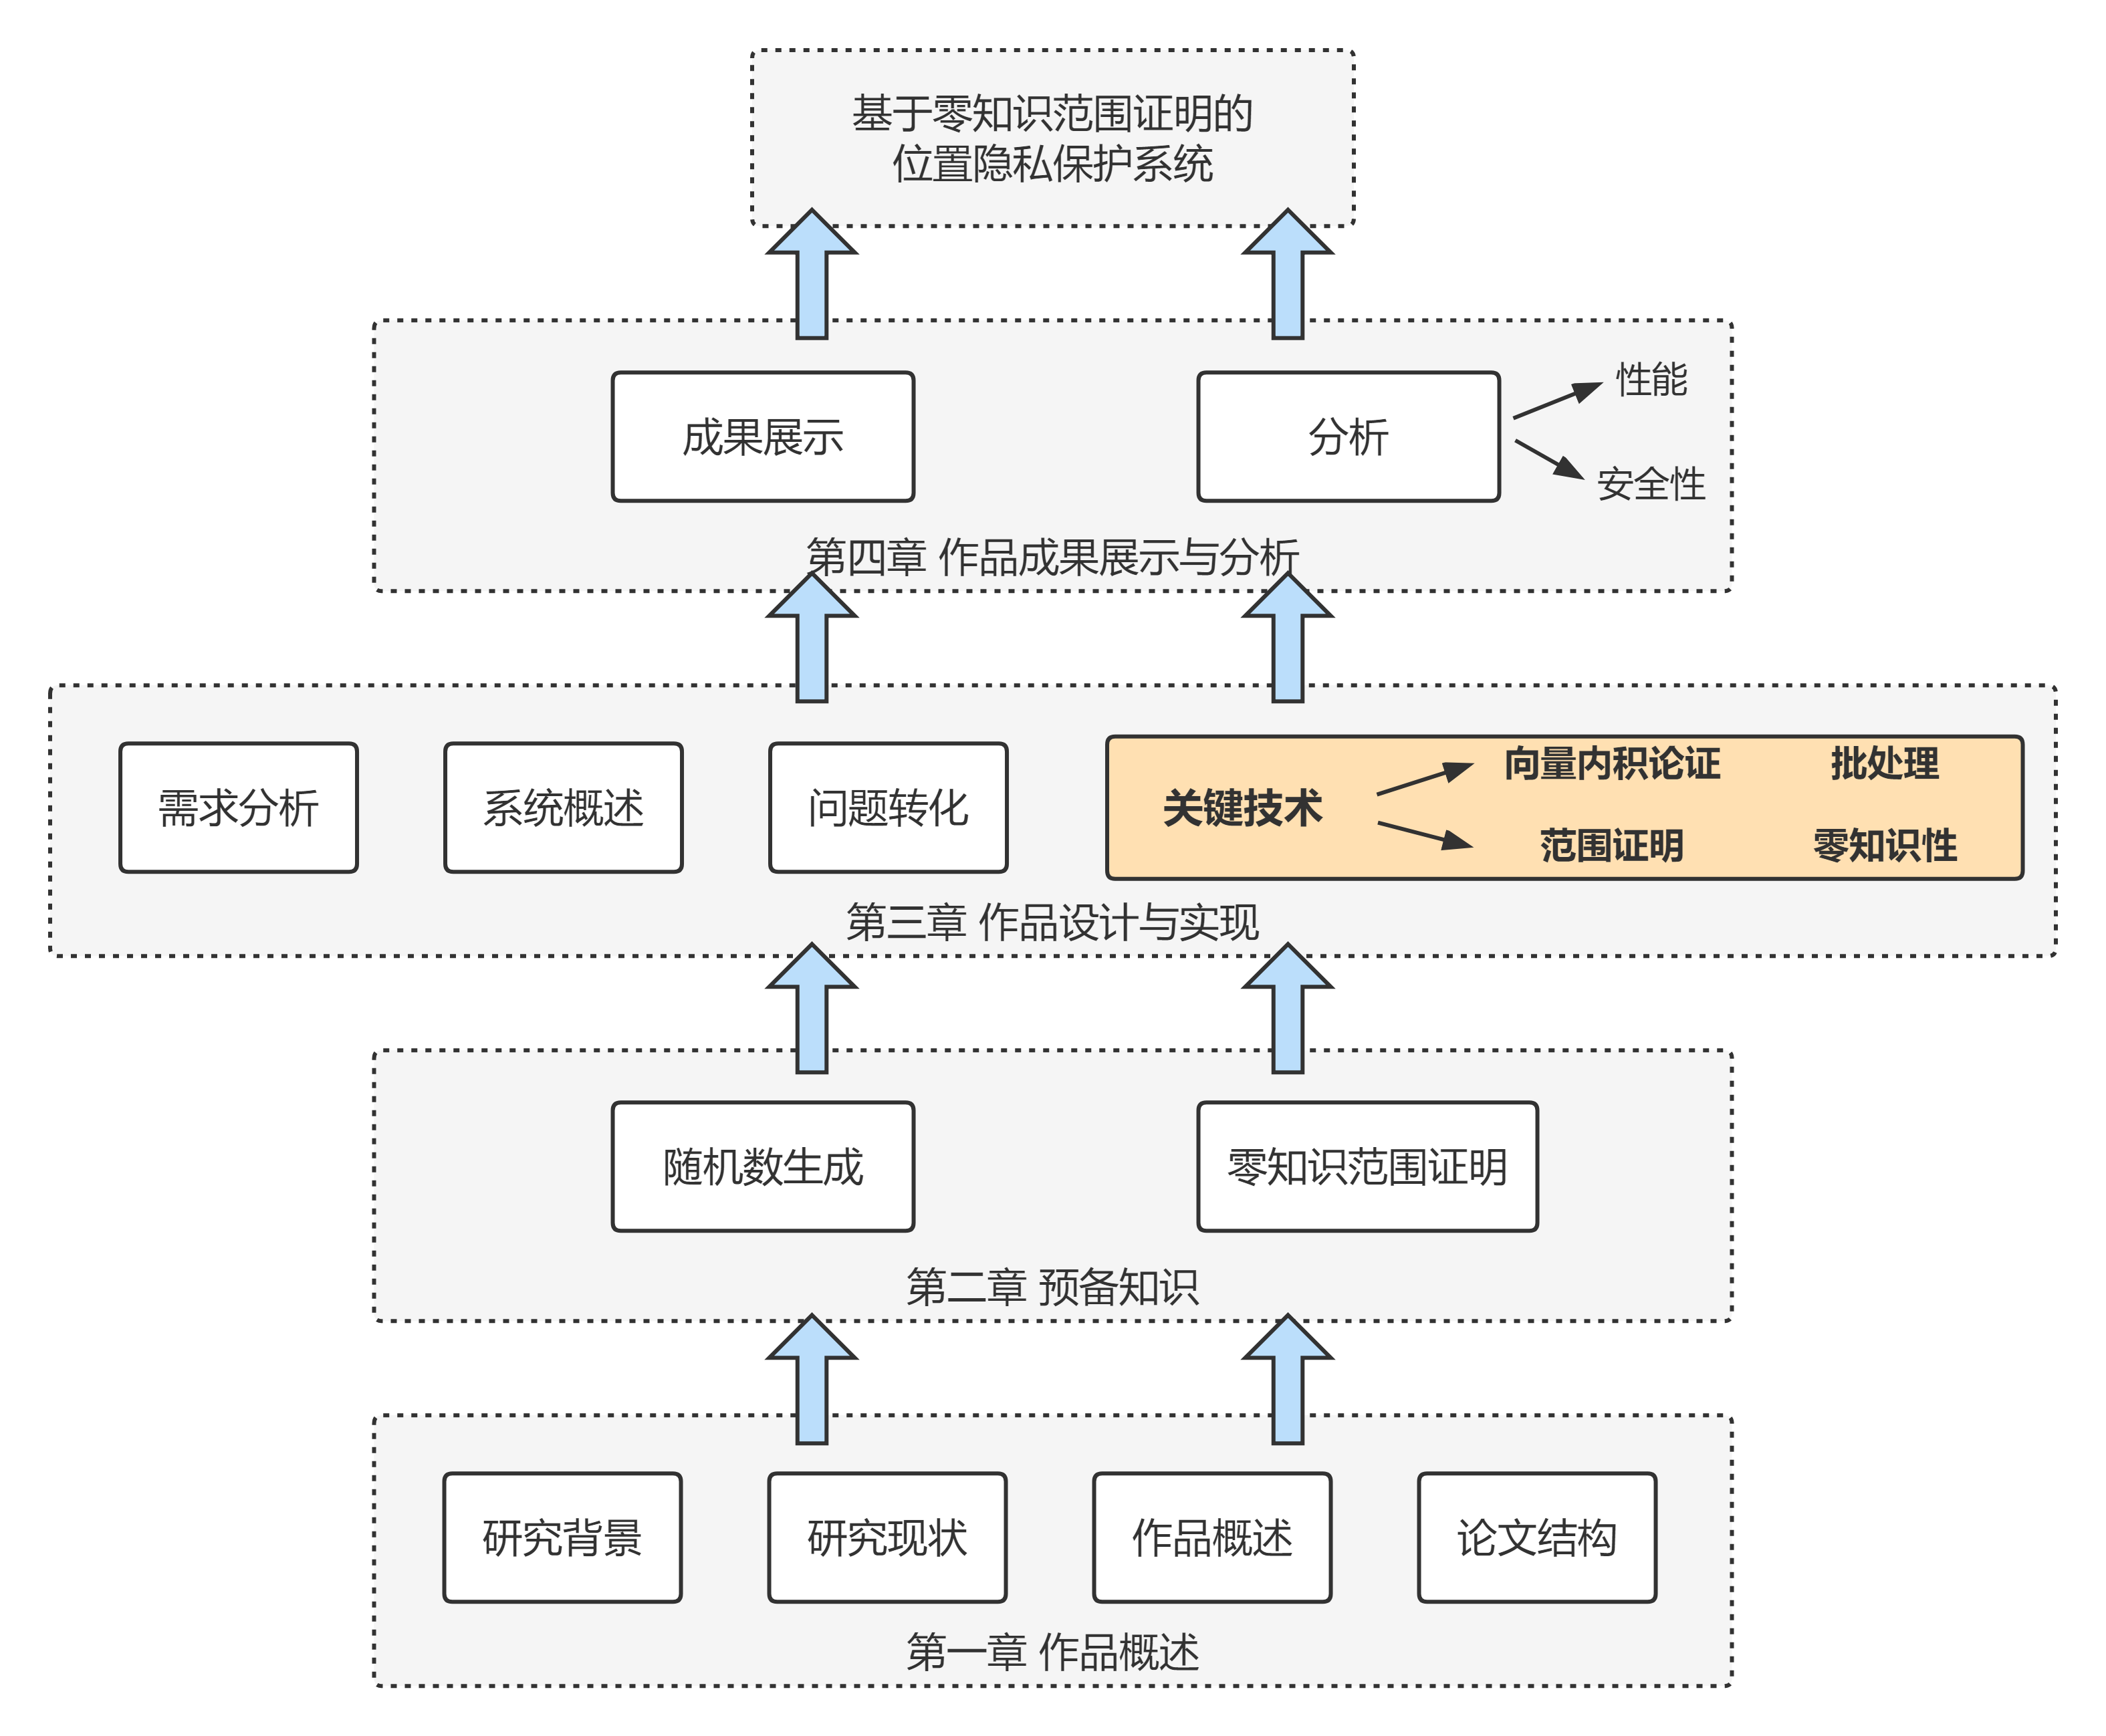
\includegraphics[width=0.9\textwidth]{./include_picture/2023冯如杯-论文组织结构} %插入图片,[]中设置图片大小,{}中是图片文件名
	\caption{论文组织结构} %最终文档中希望显示的图片标题
	\label{论文组织结构} %用于文内引用的标签
\end{figure}

\iffalse
\subsection{前景扩展(to be merged)}
兴趣点(Point of Interest)分析:【引用】
兴趣点指的是用户周边地理实体,包括餐馆酒店、娱乐场所、商超银行、地铁公交等,可能是用户潜在感兴趣的消费地点。
服务提供商通过分析用户位置的周边信息,满足用户查询需求。

社交娱乐:交友软件,同城社交分享:
同城摇一摇,同城交友

精确广告服务:
广告商通过对用户精确位置和活动轨迹的分析,向用户投放精准定制化的广告,尤其是向用户推荐周边商户和服务。
周边位置的购物折扣、餐饮娱乐和房屋租赁等广告可以很好切中用户需求,拉近周边商户与用户举例。
\fi 

%********************预备知识********************
\section{预备知识}
简单技术背景介绍
\subsection{随机数生成}

\subsection{范围证明的理论基础}
\subsubsection{默克尔树}
默克尔树\cite{Merkle}(Merkle Tree or Hash Tree)是一棵用哈希值搭建起来的树,树的所有节点都存
储了哈希值。整棵树包含根节点、中间节点和叶节点。树采取自下而上的生成方式,叶节点经
哈希运算得到哈希值,而其余节点的哈希值均由其子节点的哈希值经哈希计算得到。默克尔树
的具体结构见图\ref{Merkle}。
\begin{figure}[H]
  \centering
  \includegraphics[width=0.8\textwidth]{Merkle_tree.bmp} 
  \caption{默克尔树结构图}
  \label{Merkle}
\end{figure}
基于哈希函数的防碰撞特性(Collision resistance)、隐藏性(Hiding)和谜题
友好性(Puzzle friendly),对默克尔树的任意局部修改,都会对根节点和路径
上的中间节点产生影响。默克尔树的这个特性提供了一种很好的检测数据是否被篡
改的方法。在本文中,我们使用具有抗碰撞特性和不可逆特性的哈希函数来构造默
克尔树,进而利用构造的树来完成对向量的承诺,并通过次线性尺度的证明来开放
树的多处索引。对向量$\;v\;$的承诺包含以下三种算法,即承诺操作(Commit)、
开放操作(Open)、验证操作(Verify):
\begin{itemize}
  \item $\text{root}_v\leftarrow \text{MT.Commit}(v)$
  \item $(\{v_i\}_{i\in\mathcal{I}},\pi^v_{\mathcal{I}})\leftarrow\text{MT.Open}(\mathcal{I},v)$
  \item $\{1,0\}\leftarrow\text{MT.Verify}(\text{root}_v,\mathcal{I},\{v_i\}_{i\in\mathcal{I}},\pi^v_{\mathcal{I}})$
\end{itemize}

\subsubsection{里得·所罗门编码}
里得·所罗门编码\cite{Fourty-two}\cite{Eight}(Reed-Solomon Code, RS Code)是一种编码方式,用其编码的码字是域上
某个特定单变量多项式的一组函数值,表示成向量的形式。因此,在本文中我们使用RS\;Code来编码
向量。\par
用抽象代数的模型来定义,选择一个$\;q\;$阶的有限域$\mathbb{F}$,作为编码的字母表。
再选择$\mathbb{F}$的一个陪集$\;L\;$,所选择的特定单变量多项式成为编码多项式(encoding polynomial),且度
小于$\rho\cdot|L|$,其中$\rho\in(0,1)$称为编码率,用这样的多项式编码出的向量表示为
$\text{RS}[L,\rho]\in\mathbb{F}^{|L|}$。\par
具体而言,编码的过程如下:设插值集$H=\{\xi_1,\cdots,\xi_{|H|}\}$,估值集$L=\{\eta_1,\cdots,\eta_{|L|}\}$,
且$|L|>|H|$,被编码的向量设为$v\in\mathbb{F}^{|H|}$。首先,找到预设的度的编码多项式$\hat{p}$,使得
$\hat{p}|_H=\{\hat{p}(\xi_1),\cdots,\hat{p}(\xi_{|H|})\}=v$。然后计算$\hat{p}$在$L$上的估值(Evaluation),得到
码字$\hat{p}|_L$。计算估值和插值的算法使用快速傅里叶变换(Fast Fourier Transform, FFT)和其逆变换(Inverse FFT, IFFT)。

\subsubsection{诚实验证方前提的零知识证明}
零知识证明(Zero-Knowledge Argument of Knowledge, ZKAoK
)是一种验证协议,在其中证明方(Prover)不提供任何有关某个论断的有用信息,
而能使验证方(Verifier)验证该论断为正确的。这项协议技术
在信息安全及密码学等领域应用广泛。
“诚实验证方前提(Honest Verifier)”意为验证方是正确遵循协议进行验证的。\par
用计算复杂度理论(Computational Complexity Theory)的模型定义,零知识证明
是一个用于证明NP(Non-deterministic Polynomial)二元关系$\mathcal{R}$的
算法三元组$(\mathcal{G}, \mathcal{P}, \mathcal{V})$。其中$\mathcal{G}$表示
公共参数生成算法,设其输出为pp;$\mathcal{P}$和$\mathcal{V}$分别表示非确定多
项式时间(Probabilistic Polynomial Time, PPT)的证明算法和验证算法。\par
诚实验证方前提的零知识证明\cite{Fourty-two}具有以下条件需要满足:
\begin{itemize}
  \item \textbf{\emph{完备性(Completeness)}}:即正确的论断都可以被证明为正确。假设$\lambda$为私有参数,
      对于每个$\mathcal{G}$的输出pp$\leftarrow\mathcal{G}(1^{\lambda})$,每
      个$\mathcal{R}$中的元素$(x,\omega)$,以及字母表上任意字符串$z\in\{0,1\}^*$,有:
      \[\text{Pr}[\langle \mathcal{P}({\omega}),\mathcal{V}(z)(\text{pp},x)=1\rangle]=1-\text{negl}(\lambda)\]
      其中Pr表示概率,negl($\lambda$)表示当$\lambda$足够大时,可以忽略不计的量。
  \item \textbf{\emph{正确性(Soundness)}}:即被证明的论断大都是正确的,只有极小的可能出错。对于每个$\mathcal{G}$的输出pp
      $\leftarrow\mathcal{G}(1^{\lambda})$,
      每个不在$\mathcal{R}$中的元素$(x,\omega)$,以及字母表上任意字符串$z\in\{0,1\}^*$,有:
      \[\text{Pr}[\langle \mathcal{P}^*({\omega}),\mathcal{V}(z)(\text{pp},x)=1\rangle]\le\text{negl}(\lambda)\]
      其中$\mathcal{P}^*$表示任意的PPT证明方。
  \item \textbf{\emph{零知识性(Zero-knowledge)}}:即$\mathcal{P}$和$\mathcal{V}$之间的对话可以只依据公开信息被完全模拟。对于
      每个$\mathcal{G}$的输出pp$\leftarrow\mathcal{G}(1^{\lambda})$,任意的诚实的PPT验证方$\mathcal{V}$,
      每个$\mathcal{R}$中的元素$(x,\omega)$和任意字母表上的字符串$z\in\{0,1\}^*$,存在一个PPT模拟机$\mathcal{S}$,使得:
      \[\{\langle \mathcal{P}(\omega),\mathcal{V}(z)\rangle(\text{pp},x)\}\overset{c}{\approx}\{\mathcal{S}^{\mathcal{V}}(\text{pp},x,z)\}\]
      其中$\mathcal{S}^{\mathcal{V}}$表示多项式空间下给定$\mathcal{V}$的模拟机,$\overset{c}{\approx}$表示两者在计算上不可区分
      (Computationally indistinguishable)。
  \item \textbf{\emph{知识论证性(Argument of knowledge)}}:即所有论证的证明都不会是不合法的。对于每个$\mathcal{G}$的输出pp$\leftarrow\mathcal{G}(1^{\lambda})$,
      任意的$x,z\in\{0,1\}^*$,对于所有恶意的PPT证明方$\mathcal{P^*}$,存在一个可预期多项式时间的抽取机$\mathcal{E}$,使得:
      \[\text{Pr}[\langle \mathcal{P^*}(\omega),\mathcal{V}(z)\rangle(\text{pp},x)=1\wedge((x,\omega)\not\in\mathcal{R})|_{\omega\leftarrow\mathcal{E}^{\mathcal{P^*}}(\text{pp},x)}]\le\text{negl}(\lambda)\]
      其中$\mathcal{E}^{\mathcal{P}^*}$表示抽取机对$\mathcal{P^*}$的任意性及整个运行过程都具有访问权限。
\end{itemize}

\subsubsection{交互式谕示机证明}
交互式谕示机证明\cite{seven}\cite{Thirty-nine}(Interactive Oracle Proof, IOP)是一种证明系统模型,在其中验证方可以通过谕示机概率性地问询证明方所持有的
关于被证明的论断的有效信息,但由于是概率性地问询,所以验证方并不能得到证明方的全部信息。\par
同样,使用计算复杂度理论的模型来定义,IOP是证明$\;k\;$轮NP二元关系的算法三元组$(\mathcal{G},\mathcal{P},\mathcal{V})$,其中
$\mathcal{G}$表示公共参数生成算法,设其输出为pp;$\mathcal{P}$和$\mathcal{V}$分别表示PPT证明算法和验证算法。具体而言,一个$\;k\;$轮的IOP包含$\;k\;$
轮的交互(interaction)。在第$\;i\;$轮($0<i\le k$),验证方向证明方均匀且随机地发送消息$m_i$,且验证方能够通过谕示机得到
以$\;m_i\;$为输入的输出,证明方需返回$\;\pi_i\;$给验证方。在最后一轮,验证方得到了证明方返回的$\;k\;$个位置的信息
$\;\pi=(\pi_1,\cdots,\pi_k)$,并且需决定接受或拒绝证明方的证明(Proof)。\par
交互式谕示机证明\cite{six}具有以下条件需要满足:
\begin{itemize}
  \item \textbf{\emph{完备性(Completeness)}}:对于每个pp$\leftarrow\mathcal{G}(1^{\lambda})$以及$(x,\omega)\in\mathcal{R}$,有:
        \[\text{Pr}[\langle \mathcal{P}(\omega),\mathcal{V}^{\pi}\rangle(\text{pp},x)=1]=1\]
        其中$\mathcal{V}^{\pi}$表示$\mathcal{V}$可以访问谕示$\pi$。
  \item \textbf{\emph{正确性(Soundness)}}:对于每个pp$\leftarrow\mathcal{G}(1^{\lambda})$,每个PPT的$\mathcal{P^*}$以及$(x,\omega)\not\in\mathcal{R}$,有:
        \[\text{Pr}[\langle \mathcal{P}^*(\omega),\mathcal{V}^{\pi}\rangle(\text{pp},x)=1]\le\text{negl}(\lambda)\]
\end{itemize}\par
在本文中,主要涉及两种类型的IOP,分别是\emph{RS-IOP}和\emph{IOP of proximity},前者即使用里德-所罗门码(Reed-Solomon code)的IOP,
后者指对于正确性的条件,允许证明方的秘密和合法证据之间具有微小的差距(proximity)。

\subsubsection{单变量求和校验协议}
单变量求和校验协议(Univariate Sum-check Protocol)主要应用于有限域上的多项式求和问题。首先,假设有两个乘法群
$H, L\subset \mathbb{F}\;(|L|>|H|)$,一个小于$k(k>|H|)$阶的单变量多项式$f(\cdot)$,以及一个被声明(claimed)的和$\mu$。
在已有假设上,单变量求和校验协议的作用就是证明$\sum_{a\in H}f(a)=\mu$。\par
在实际操作中,证明方需要将$f(x)$利用带余除法唯一地转化为$x\cdot\hat{p}(x)+\zeta+\hat{Z_H}(x)\hat{h}(x)$,
其中除式为$\hat{Z_H}(x)$,代表$H$上的“消失”多项式(Vanishing polynomial),满足$\forall a\in H,\;\hat{Z_H}(a)=0$。
接着,基于对$\hat{f}|_L$和$\hat{h}|_L$的谕示机访问,验证方可以验证是否有$\hat{p}|_L\in\text{RS}(L,\frac{|H|-1}{|L|})$
以及$\hat{h}|_L\in\text{RS}(L,\frac{|L|-|H|}{|L|})$,其中:
\begin{equation}\hat{p}(x)=\dfrac{|H|\cdot\hat{f}(x)-\mu-|H|\cdot\hat{Z_H}(x)\hat{h}(x)}{x}\end{equation}
以上采用RS编码的IOP满足正确性和完备性\cite{six},当我们将它转换为一个标准IOP时,它仍然是在检验
谕示$\hat{f}|_L,\hat{h}|_L,\hat{p}|_L$是否为具有相应
度的界限的RS码。而这个过程可以通过下面的低度检测协议来完成。

\subsubsection{低度检测和FRI}
给定度$k_1,\cdots,k_t$,码字$\hat{v}_1|_L,\cdots,\hat{v}_t|_L$,其中$L$为一个乘法陪集,低度检测协议允许验证方借助对这些码字的谕示机访问来检验以下语句是否成立:
\begin{equation}\forall j\in\{0,\cdots,t\},\;\hat{v}_j|_L\in\text{RS}[L,\frac{k_j}{|L|}]\label{低度检测}\end{equation}\par
公式(\ref{低度检测})用于检测编码给定码字的编码多项式的度是否低于给定的度。\par
在本文中,我们的低度检测协议选取快速Reed-Solomon交互式谕示机邻近证明\cite{three}(Fast Reed-Solomon Interactive Oracle Proof of Proximity, Fast RS IOPP, FRI)。
给定对证明方消息$\;l\;$处取值的谕示机访问,该FRI 是具有完整性(Completeness)和正确性(Soundness)容错率为
$O(\frac{L}{\mathbb{F}})+\text{negl}(l,k)$的IOPP,其中$l=O(\lambda),k=\max\{k_1,\cdots,k_t\}$。\par
总的来说,用于实现单变量求和校验的FRI协议可以表示为:
\begin{equation}\langle \text{FRI}.\mathcal{P}(\hat{f},\hat{h},\hat{p},\text{FRI}.\mathcal{V}^{\hat{f}|_L,\hat{h}|_L,\hat{p}|_L})\rangle(k,k-|H|,|H|-1)\end{equation}\par

\subsubsection{向量内积论证}
向量内积论证(Inner Product Arguments, IPA),是一
证明手段,即给出两个向量$\vec{a},\vec{b}$的承诺
(commitment),其中$\vec{a},\vec{b}$属于
$\mathbb{F}^n$,$\mathbb{F}$为域,可以证明这两个
被承诺的向量的内积等于某一公开的标量,而不需要揭示
这两个向量的具体取值。\par
在信息安全领域,常见的承诺方式有皮特森哈希值
(Pedersen hash)或者RS编码,在本文中采用后者。\par
向量内积论证可以用于证明单变量多项式在某点处的值。首先将多项式
$\hat{f}=f_0+f_1x+\cdots+f_nx^n$表示为向量$\vec{f}=(f_0,f_1,\cdots,f_n)$
注意到:
\begin{equation}\hat{f}(s)=(\vec{f},(1,s,\cdots,s^n))\label{IPA转化}\end{equation}\par
公式(\ref{IPA转化})表明计算等价于两个向量的内积,因此可转化为向量内积论证。




%********************作品设计与实现********************
\section{作品设计与实现}

\subsection{需求分析}
为了使改进后的位置隐私保护系统更符合当前应用市场的需要,本文设计出的作品应满足一定的功能和性能的需求。本节将对位置隐私保护系统在功能上、性能上的需求进行分析,从而为本文作品指引改进方向。

\subsubsection{功能需求}
位置隐私保护系统涉及用户、服务提供商乃至第三方应用,具有广泛的应用场景。因此,改进后的位置隐私保护系统应满足一定的功能需求,以满足各方需要。
\par 
\textbf{(1)保护用户位置隐私安全}
\par 
位置隐私保护系统的出发点是保护用户隐私安全,不管如何改进,这一点应当始终保持。当前位置隐私保护技术主要通过添加虚假或者无关的位置信息,以此混淆用户真实的位置信息。改进后的位置信息保护系统虽然是基于零知识范围证明技术,但也应该达到这一效果。
\par 
\textbf{(2)保证用户返回的位置信息可信}
\par 
虽然在现阶段的“用户-服务提供商”模式下,保证用户提交的位置信息的真实性似乎没有很大的必要,但是可以看到,攻击者可以通过向服务提供商或者系统提交错误的位置信息,窃取系统信息,从而达到某种攻击系统的目的。所以改进后的位置隐私保护系统也应该保证位置信息的真实性,防止攻击者通过提交错误的位置信息攻击系统这一漏洞。
\par 
\textbf{(3)保障用户得到的服务质量}
\par 
用户的位置隐私固然重要,但是保护用户隐私应该在不明显影响用户得到的服务质量这一前提下。现有的K-匿名技术、虚假位置技术等位置隐私保护技术都能大致满足这一需求。因此,改进后的位置隐私保护系统也应该满足这一需求。

\subsubsection{性能需求}
考虑到用户所在的移动用户端性能有限,以及系统的计算开销应该限制在一定范围内,实际应用中位置隐私保护系统应该满足一定的性能需求。
\par 
\textbf{(1)计算复杂度}
\par 
通常用户发起查询请求后,服务提供商应该在较短时间内返回查询结果和对应服务。同时,用户所在的移动用户端计算、存储能力通常比较有限,难以支撑复杂的计算过程。所以改进后的位置隐私保护系统应该具有较低的计算时间、空间复杂度,从而保证系统实际运行的效果。
\par 
\textbf{(2)可拓展性}
\par 
近年来我国位置服务产业快速发展,截至2021年卫星导航与位置服务产业总体产值已经达到4690亿元\cite{czh_5.1},产业前景不可估量。在此背景下,位置隐私保护系统将会面向多种应用场景,这也对位置隐私保护系统的可拓展性提出了比较高的要求。所以改进后的系统在设计和实现上需要有一定程度的解耦、分层设计,以适应随时变化的业务场景。所以在设计系统时应有意识地将系统模块化开发,并留下优化、拓展的空间,便于新功能的拓展。
\par 
\textbf{(3)健壮性}
\par 
位置信息涉及用户隐私,应该防止泄露的可能。所以系统应该具有一定的防卫或者恢复能力,在受到攻击或者发生错误时能采取措施减少损失。具体而言,当局部系统出错或受到攻击时,这部分系统应该能在较短时间内恢复并继续运行,而不会造成大范围影响,从而在最大程度上减少系统运行的风险。这也是应用场景对位置隐私保护系统在健壮性上的要求。


\subsection{系统概述}
本作品系统主要涉及两个主体:服务请求方和服务提供商。
服务请求方一端由\textbf{手机网页端交互界面、定位与生成零知识范围证明系统}构成,具体技术涉及 Vue.js 、C++ 和 Python。
服务提供商一端由\textbf{数据库、(零知识范围证明)验证系统}构成,开发技术使用 Shell 和 MySQL 。
\par
系统工作总体流程图如图所示 \ref{flowchart}。首先,请求方选择以何种精度 r 模糊自己的位置,接着本地系统自动采集用户的精确经纬度地理位置 $(x, y)$ 。
本地系统获得参数 $(x, y, r)$ 后,在以 $\frac{r}{2}$ 为半径的圆内, 生成一个模糊位置 $(x',y')$ 。
具体模糊位置生成过程为,使用基于椭圆曲线的轻量随机数生成算法(见预备知识节:3.2??),生成一个随机极坐标 $(R, \alpha)$ ,极坐标原点为 $(x,y)$ 。然后基于该相对极坐标计算出模糊位置 $(x',y')$ 。
\par
本地系统基于该模糊位置 $(x',\ y',\ R)$ ,生成一个对范围的零知识证明:$Proof: R<\frac{r}{2}$ ,并将 $x,\ y,\ Proof$ 打包发送至服务提供商数据库。
服务提供商验证证明,确认用户在该模糊范围内,提供相应的服务。
最终效果是服务提供商只知道请求方在 $(x',y',\frac{r}{2})$ 这一个圆形范围内,服务请求方保护了自身位置隐私,同时其接受的服务精度偏差不超过 $r$。
%系统工作流程图
\begin{figure}[H] %H为当前位置,!htb为忽略美学标准,htbp为浮动图形
    \centering %图片居中
    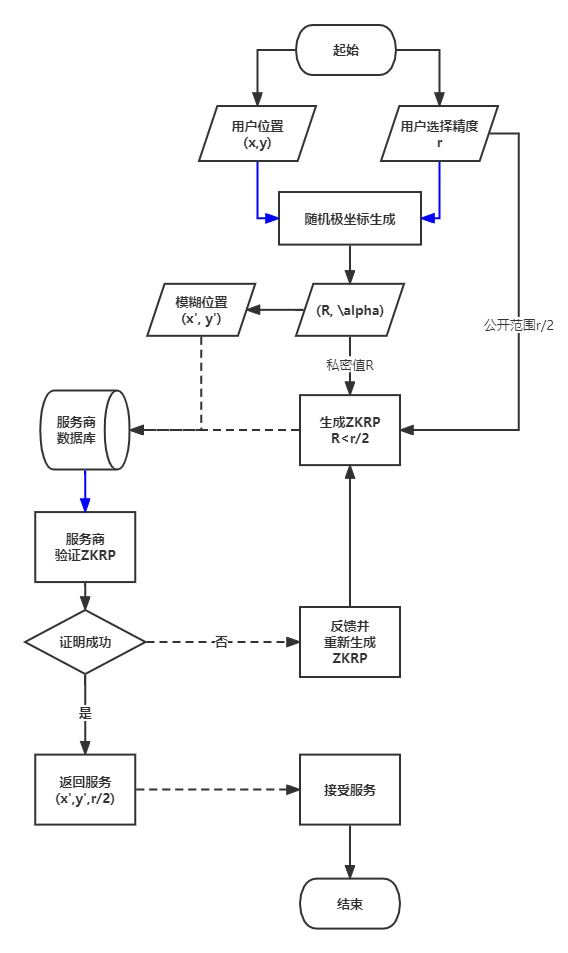
\includegraphics[width=0.6\textwidth]{系统工作流程图.jpg} %插入图片,[]中设置图片大小,{}中是图片文件名
    \caption{系统工作总体流程图} %最终文档中希望显示的图片标题
    \label{flowchart} %用于文内引用的标签
\end{figure}

基于零知识范围证明的的位置隐私保护系统改进实际上是围绕GPS上的零知识范围证明展开的。
这是改进的新系统的技术核心,只要能实现这一点,整体的系统便能搭建起来。为了使系统的
针对目标更加清晰,我们定义如下问题场景:证明方在拥有一个隐藏的用户GPS坐标和一个公开
的参考点GPS坐标的基础上,向验证方证明用户GPS坐标在参考点GPS坐标的一定范围内,但这
个过程不会透露用户GPS坐标的具体信息。在以下两章中,我们将介绍该问题的解决方案和相
应的技术原理。
\subsection{基于哈达玛积的问题转化}
观察问题场景,我们发现其中涉及两个GPS坐标:隐藏的用户GPS坐标和公开的参考点GPS坐标,
分别记作$S(x_1,y_1)$和$P(x_2,y_2)$。考虑到实际生活场景中的GPS坐标往往是经纬度形式
,因此这两个坐标同样采用经纬度形式。同时为了兼顾一定的准确性,在经纬度精度上,本文选
取4位小数作为参考样例,即$x_1$,$x_2$,$y_1$,$y_2$均为五位小数。此时最大误差大概是
在$5$米左右。当然,如果需要让结果进一步精确,仍可以进一步调整精度。\par
要判断坐标$S$是否在坐标$P$的一定范围内,我们可以参考平面中心圆模型。通过判断两者间的
距离$R$是否处于一定数值范围内,即可检验坐标间关系是否满足要求。为了使问题更加明确,
本文中用符号$l_{\min}$,$l_{\max}$分别来表示距离的下界和上界,且均为整数。其中整数的
选取主要为了更好地运用零知识范围证明。实际应用中,$l_{\min}$,$l_{\max}$应根据具体需
求进行一定的变化。基于以上定义,我们将问题转化为:用户GPS坐标在参考点GPS坐标的一定
范围内等价于检验以下公式
\begin{equation}l_{\min}< d_{SP}\leq l_{\max}\end{equation}\par
其中$d_{SP}$代表坐标$S$和$P$之间的距离,数值选取小数点后5位。而要得出$d_{SP}$的具
体数值,我们需要利用坐标$S(x_1,y_1)$和$P(x_2,y_2)$进行如下公式计算:
\begin{equation}
  \begin{cases}
    &S^{\prime}=(R\cos x_1\cos y_1,R\sin x_1\cos y_1,R\sin y_1),\\
    &P^{\prime}=(R\cos x_2\cos y_2,R\sin x_2\cos y_2,R\sin y_2),\\
    &d_{SP}=R\arccos[\cos(x_1-x_2)\cos y_1\cos y_2+\sin y_1\sin y_2].
  \end{cases}
\end{equation}\par
其中$S^{\prime}$和$P^{\prime}$分别代表经纬度坐标$S(x_1,y_1)$
和$P(x_2,y_2)$在三维直角坐标系下对应坐标,$R$代表地球的半径。这样
就可以进行$d_{SP}$和$L$的比较了。\par
但是,我们采用的零知识范围证明适用于任意整数范围,而非任意实数范围。
并且零知识范围证明主要是对向量进行操作,而非直接的数值。因此我们不仅
需要将$d_{SP}$进行整数化处理,还要进一步将其转化为进制形式来形成对应
向量。下面介绍解决方案。\par
首先,将$d_{SP}$,$l_{\min}$,$l_{\max}$乘以$10^5$,进一步得
到$D_{SP}$,$L_{\min}$,$L_{\max}$这样我们不仅保留了小数部分,
避免了直接去除小数部分带来的误差,同时完成了取整。不过值得注
意,乘以$10$的几次方主要取决于应用需求和相关参数的精度选取。\par
接着,取满足$u^{n-1}<L_{\max}\leq u^n$的
$u$和$n$,对$D_{SP}$,$L_{\min}$,$L_{\max}$,$D_{SP}-L_{\min}$,$D_{SP}-L_{\max}+u^n$
分别进行进制转化,得到向量$v$,$a$,$b$,$c$,$d$。
本文中以二进制作为参考样例。进一步计算以下内积关系,以证明$L_{\min}< D_{SP}\leq L_{\max}$:
\begin{equation}
  \begin{cases}
    &\langle v\odot(v-1^m),r\rangle=0\\
    &\langle c\odot(c-1^m),r\rangle=0\\
    &\langle d\odot(d-1^m),r\rangle=0\\
    &\langle c,r_{[:m-n]}||0^n\rangle=0\\
    &\langle d,r_{[:m-n]}||0^n\rangle=0\\
    &\langle v-a-c,2^m\rangle=0\\
    &\langle v-b+bi(2^n)-d,2^m\rangle=0
  \end{cases}
\end{equation}
\par
以上运算基于一个足够大的有限域$\mathbb{F}$的。参数$m$大小为$|\mathbb{F}|$,
参数$r$是验证方随机选取的一个挑战值。$\odot$表示哈达玛积,即
$a\odot b=(a_1,\ldots,a_k)\odot(b_1,\ldots,b_k)=(a_1b_1,\ldots,a_kb_k)$。$bi()$
表示将数转化为二进制的向量。以上的七个公式就是零知识范围证明实
际上的证明对象,至此问题已经转化完成,接下去的流程就是零知识范
围证明了。其中的具体原理,详见下一章关于零知识范围证明的介绍。


\subsection{关键技术}

基于交互式谕示机证明的零知识范围证明
% +说明
\subsubsection{批处理向量内积论证}
为了实现批处理IPA(Batch Inner Product Argument, B-IPA),我们考虑单变量求和校验协议的
一个性质:无论多个多项式的阶数是否相同,单变量求
和校验协议都支持校验每一个一元多项式的和\cite{six}。此性质
为构造一个校验编码向量间内积关系的IPA提供了一种
可能,其中编码向量来自于不同阶数的编码多项式。\par
特别地,将阶数分别为$k_1,...,k_t$的秘密编码多项式
设为$\hat{v}_1,...,\hat{v}_t$。再将阶数分别为
$k_{t+1},...,k_{2t}$的公开多项式设为
$\hat{r}_1,...,\hat{r}_t$。假定证明方$\mathcal{P}$
想要证明对于任意$j \in \{1,\cdots,t\}$,都满足
$\sum_{a\in H}\hat{v}_j(a)\cdot\hat{r}_j(a)=y_j$。
实现过程中,证明方$\mathcal{P}$首先需要用默克尔
树生成对$(\hat{v}_1|_L,...,\hat{v}_t|_L)$的承
诺,并将其发送给验证方$\mathcal{V}$。接着,验证方选
择随机$t$个元素$\beta_1,...,\beta_t$,设
$\hat{q}=\sum\limits_{j=1}^t\beta_j\hat{v}_j\cdot\hat{r}_j$。
最后证明方$\mathcal{P}$和验证方$\mathcal{V}$
使用单变量求和校验协议来证明以下等式成立:
\begin{equation}\sum_{a\in H}\hat{q}(a)=\sum_{a\in H}\sum\limits_{j=1}^t\beta_j\hat{v}_j(a)\cdot\hat{r}_j(a)=\sum\limits_{j=1}^t\beta_jy_j\label{B-IPA和校验}\end{equation}\par
除此之外,批处理IPA的正确性容错率(Soundness error)仅取决于$\;t\;$个项
中最大的阶数$k_{\max}$,$k_{\max}=\max\{k_i+k_{t+i}\}_{1\le i\le t}$。\par
基于此,我们给出\textbf{批处理内积关系\emph{(Batch inner product relation)}}的定义:设二元关系$\mathcal{R}_{\text{B-IPA}}$为所有$(x,\omega)$的集合,其中:
\[\begin{aligned}&x=(\mathbb{F},H,L,\{k_j\}_{1\le j\le2t},\{\hat{r}_j\}_{1\le j\le t},\{y_j\}_{1\le j\le t})\\&\omega=\{\hat{v}_j\}_{1\le j\le t}\end{aligned}\]\par
且有公式(\ref{B-IPA和校验})成立。\par
接下来验证该批处理IPA的正确性、完备性以及知识论证性:\par
\begin{itemize}
  \item \textbf{批处理IPA的完备性\emph{(B-IPA Completeness)}}:考虑$\hat{q}$的变换,
        设对$j \in\{1,\cdots,t\}$,有$\sum_{a\in H}\beta_jv_j(a)r_j(a)=\beta_jy_j$,那么公式(\ref{B-IPA和校验})成立。
        这符合单变量和校验的二元关系形式。因此,批处理IPA有着与单变量和校验协议相同的完备性。
  \item \textbf{批处理IPA的正确性\emph{(B-IPA Soundness)}}:可以考虑以下两种发生错误的情形:\par
        \underline{情形一}.假设由于随机的线性选择组合,非法的单变量和校验关系恰好成立。
        我们假设$\forall j \in\{1,\cdots,t\},\sum_{a\in H}\hat{v}_j(a)\cdot\hat{r}_j(a)=y_j^{\prime}$
        ,且对于$\{1,\cdots,t\}$的某个子集$Q$,有$\forall q \in Q,y_q\neq y_q^{\prime}$。简便起见,不妨设$t\in Q$。
        验证方随机选择t-1个元素$\beta_1,\cdots,\beta_{t-1}$,则$\sum_{j=1}^t\beta_jy_j=\sum_{j=1}^t\beta_jy_j^{\prime}$
        当且仅当:
        \begin{equation}\beta_t=\dfrac{\beta_1(y_1^{\prime}-y_1)+\cdots+\beta_{t-1}(y_{t-1}^{\prime}-y_{t-1})}{y_t-y_t^{\prime}} \label{错误情形一}\end{equation}
        公式(\ref{错误情形一})发生的可能性仅为$1/|\mathbb{F}|$,而实际选用的有限域大小往往很大,因此概率可忽略不计。\par
        \underline{情形二}.假设变量和校验关系是非法的,即公式(\ref{B-IPA和校验})不成立。
          那么批处理IPA正确性的错误有以下三种可能:\par
        (1)若RS编码的IOP非法,则正确性取决于单变量和校验协议,故具有正确性。\par
        (2)若FRI非法,则正确性错误的上界为$\epsilon_{FRI}=\mathcal{O}(|L|/|\mathrm{F}|)+negl(\ell,k_{max}/|L|)$。\par
        (3)若默克尔树的根不正确或任意验证路径不正确,由于哈希函数的防碰撞性质,正确性错误的上界为$negl(\lambda)$。
  \item \textbf{批处理IPA的知识论证性\emph{(B-IPA Knowledge Argument)}}:批处理IPA是基于随机谕示机模型的一种知识论证。
        对于任意PPT对手$\mathcal{P}^\ast$,总存在一个PPT抽取机$\mathcal{E}$使得:给定$\mathcal{P}^\ast$的随机访问带,
        对每个由$\mathcal{P}^\ast$生成的陈述:
        \begin{equation}
          x=(\mathbb{F},H,L,\{k_j\}_{j\in [2t]},\{\hat{r_j}\}_{j\in [t]},\{y_j\}_{j \in [t]})
        \end{equation}\par
        有以下的概率为$\text{negl}(\lambda)$:
        \begin{equation}
          \text{Pr}\left[\begin{matrix}&\text{root}^*\leftarrow\mathcal{P}^*(1^{\lambda},x),\langle\mathcal{P}^*,\mathcal{V}\rangle(\text{pp,x})=1,\{\hat{v}_j\}_{1\le j\le t}\leftarrow\mathcal{E}(1^{\lambda},x):\\&\text{MT.Commit}(\mathbb{V}|_L)\neq\text{root}^*\vee(x,\{\hat{v}_j\}_{1\le j\le t})\not\in\mathcal{R}_{\text{B-IPA}}\end{matrix}\right]
        \end{equation}
        批处理IPA的知识论证属性来源于默克尔树的可抽取性。给定默克尔树树根和足够多的验证通路,总存在一个高效的方法
        能够抽取默克尔树上所有被承诺的叶节点。一旦这些叶节点被成功提取,就能通过IFFT算法获取满足$|L|>k_{\max}$的
        秘密多项式,进而实现知识论证的属性\cite{seven}\cite{Fourty-two}。
\end{itemize}\par
图\ref{B-IPA流程} 展示了在批处理IPA中,证明方与验证方进行交互、证明方向验证方证明$(x,\omega)\in\mathcal{R}_{\text{B-IPA}}$
的流程。\par
其中$\mathbb{V}|_L\in\mathbb{F}^{t\times|L|}$表示
矩阵$(a_{ij})_{t\times|L|}=(\hat{v}_i|_L[j])$。$\text{MT.Commit}(\mathbb{V}|_L)$表示将矩阵$\mathbb{V}|_L$的每一列放入
默克尔树的叶节点。
\begin{figure}[H]
  \centering
  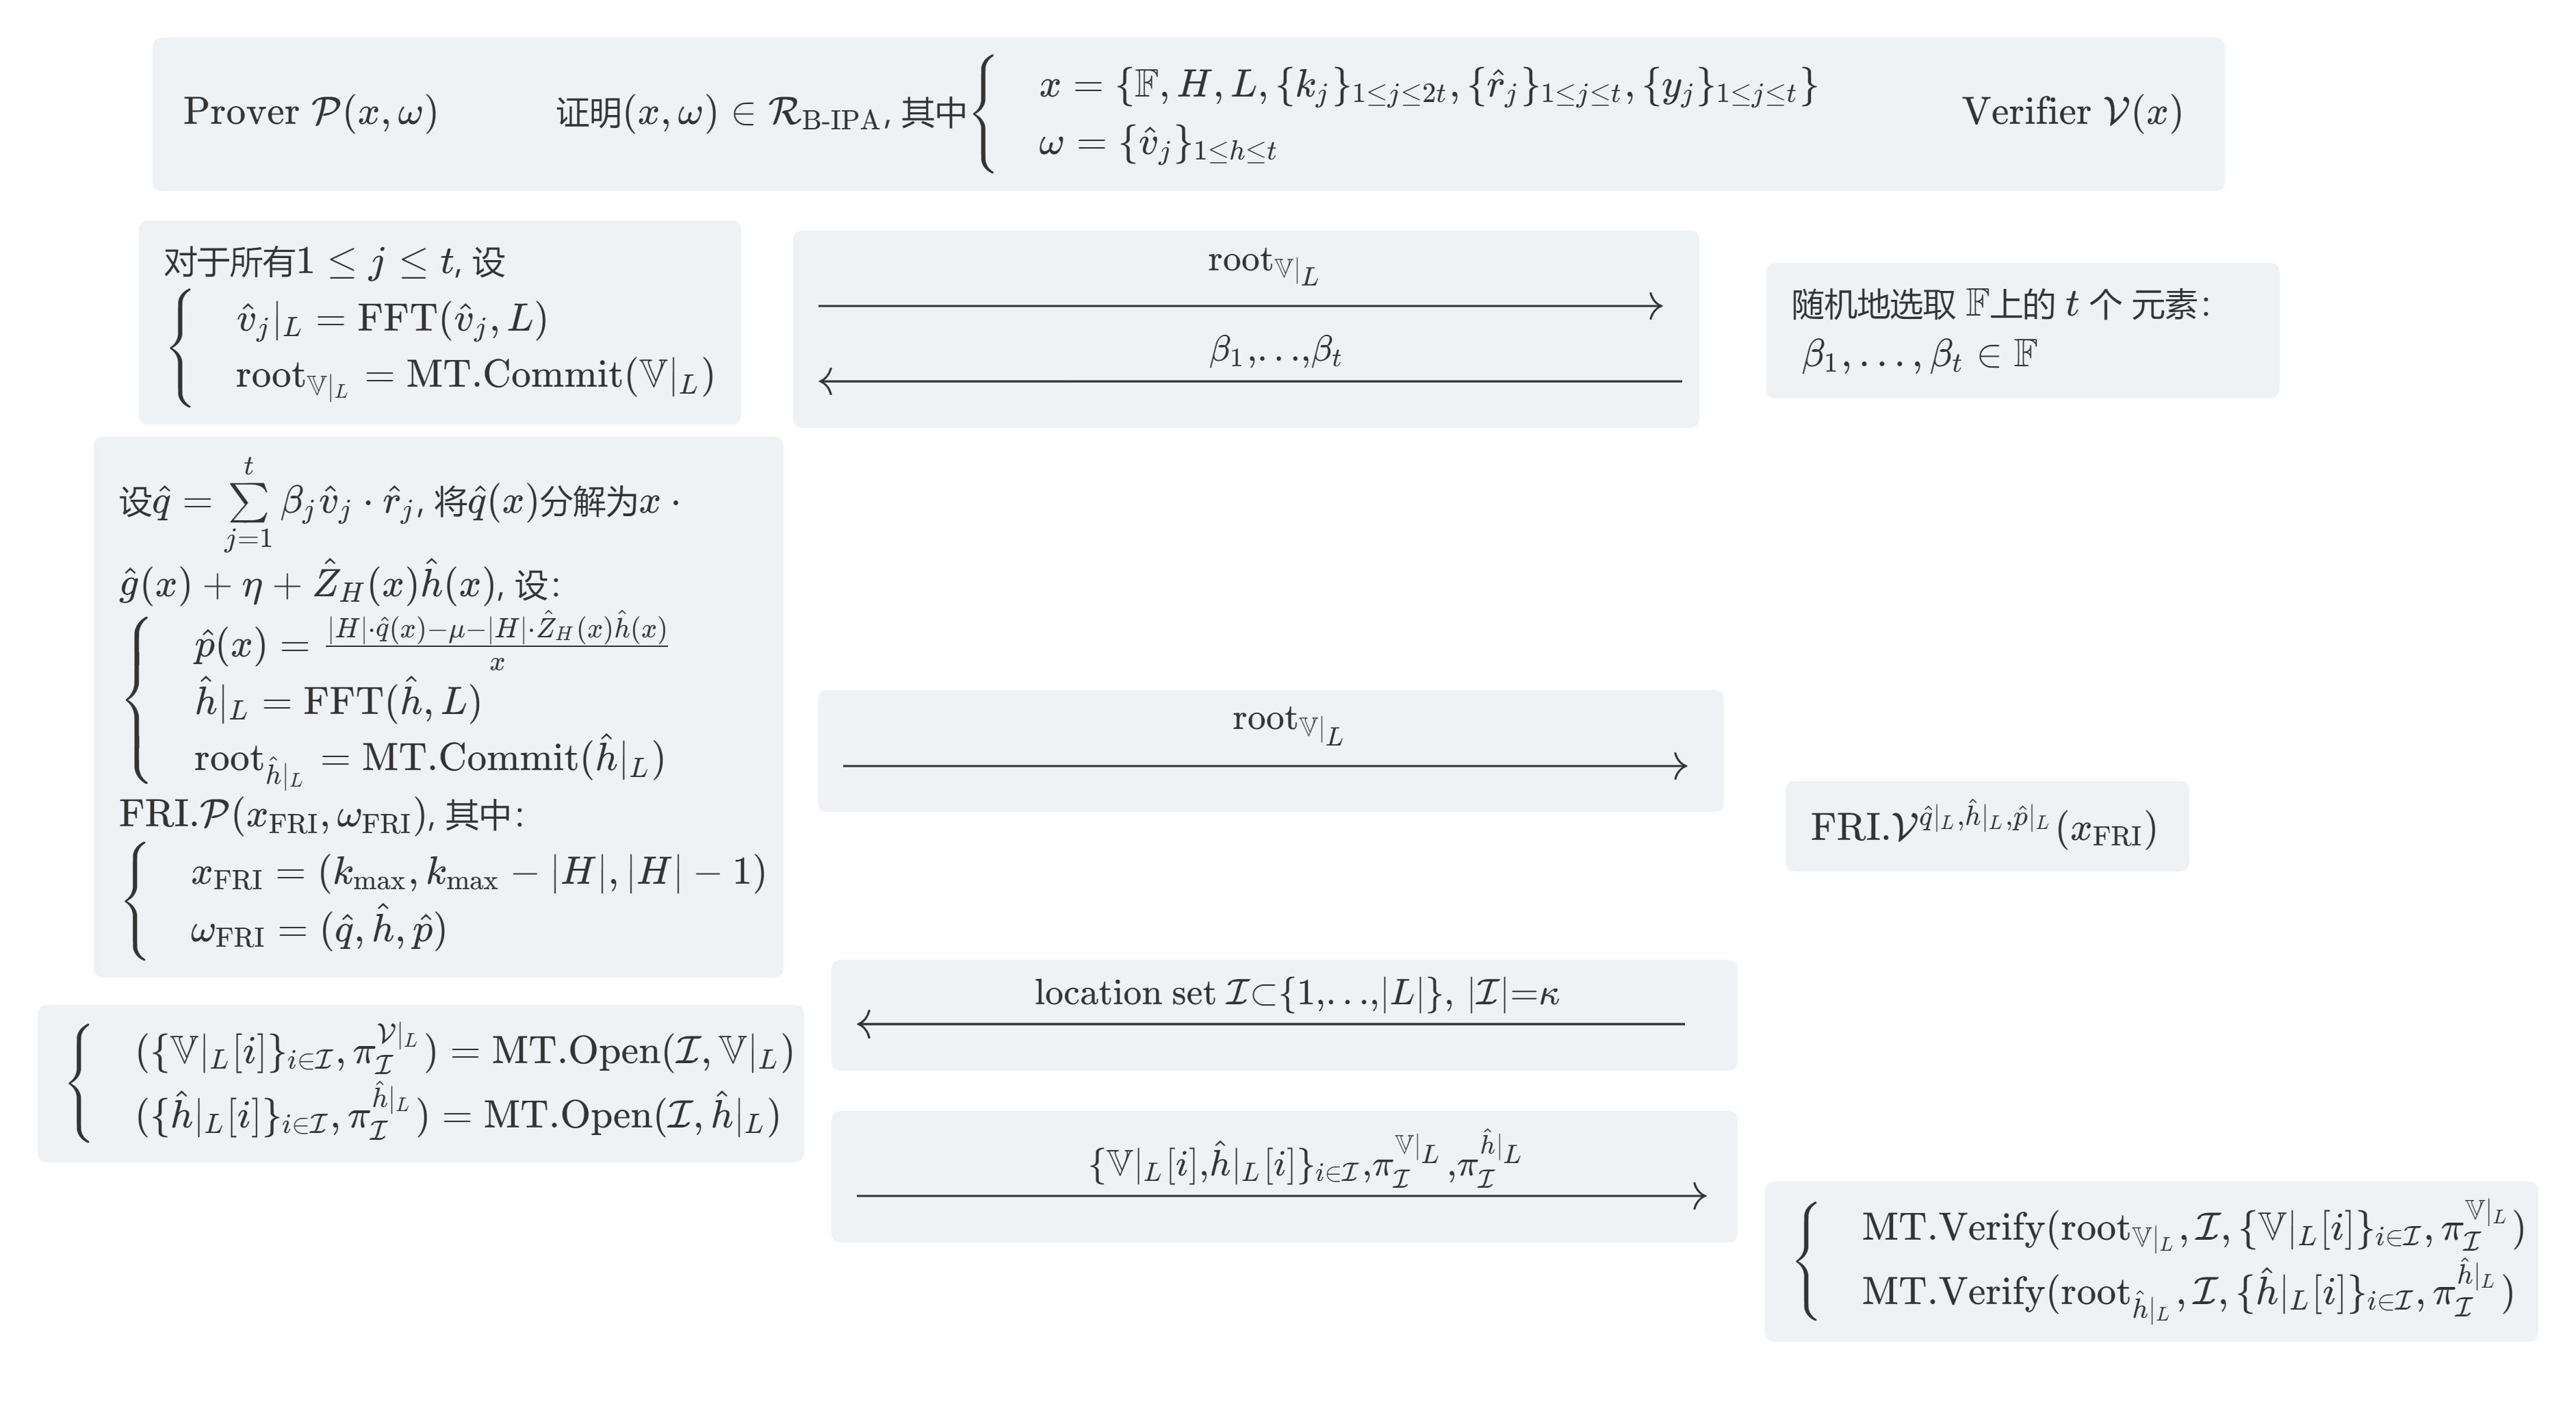
\includegraphics[width=0.85\textwidth]{./include_picture/B-IPA.png}
  \caption{: 批处理向量内积论证(Batch IPA)$\langle \text{IPA}_B.\mathcal{P}(\omega),\text{IPA}_B.\mathcal{V}\rangle(x)$}
  \label{B-IPA流程}
\end{figure}

\subsubsection{对于$[0,u^{n-1}]$的范围证明}
为了证明上界为$u^m$(即$u$进制展开为$m$位)的秘密值$V$在
范围$[0,2^n-1]$中($n<m$),只需要满足以下等式:
\begin{equation}
  \begin{aligned}
    &v\odot(v-1^m)\odot\cdots\odot(v-u^m)=0^m,\\
    &v\odot(1^{m-n}||0^n)=0^m.
  \end{aligned}
\end{equation}\par
其中$v=(v_0,v_1,\ldots,v_{m-1}),V=\sum\limits_{j=0}^mv_ju^j$。进一步地,相当于证明:
\begin{equation}
  \begin{aligned}
    &\langle v\odot(v-1^m)\odot\cdots\odot(v-u^m),r\rangle=0,\\
    &\langle v,r_{[:m-n]}||0^n\rangle=0.
    \label{任意基底范围证明}
  \end{aligned}
\end{equation}\par
经理论计算,对于验证方选取的任意$r\in\mathbb{F}$,公式(\ref{任意基底范围证明})非法成立,即出现正确性错误的概率为$1/\mathbb{F}$。\par
对于公式(\ref{任意基底范围证明}),可以利用批处理IPA来证明,即输入设为:
\begin{equation}
  \begin{aligned}
    &x=(\mathbb{F},H,L,(u|H|-(u-1)),|H|,|H|,|H|,(\hat{r},\hat{s}),(0,0)),\\
    &\omega=(\hat{w},\hat{v})
  \end{aligned}
\end{equation}\par
基于此,我们给出\textbf{范围关系\emph{(Range relation)}}的定义:设二元关系$\mathcal{R}_{\text{RP}}$为
所有$(x,\omega)$的集合,其中:
\[
  x=(\mathbb{F},H,L,m,n,[0,u^n-1]),\;\omega=V.
\]\par
且有秘密值$V$满足$V\in[0,u^n-1]$成立。\par
图(\ref{RP流程})展示了在RP中,证明方与验证方进行交互、证明方向验证方证明
$(x,\omega)\in\mathcal{R}_{\text{RP}}$的流程。其中$\mathbb{F}$是一个有限域,
$L,H$是$\mathbb{F}$的乘法陪集。秘密值$V$满足$V\in[0,u^n-1]$。
\begin{figure}[H]
  \centering
  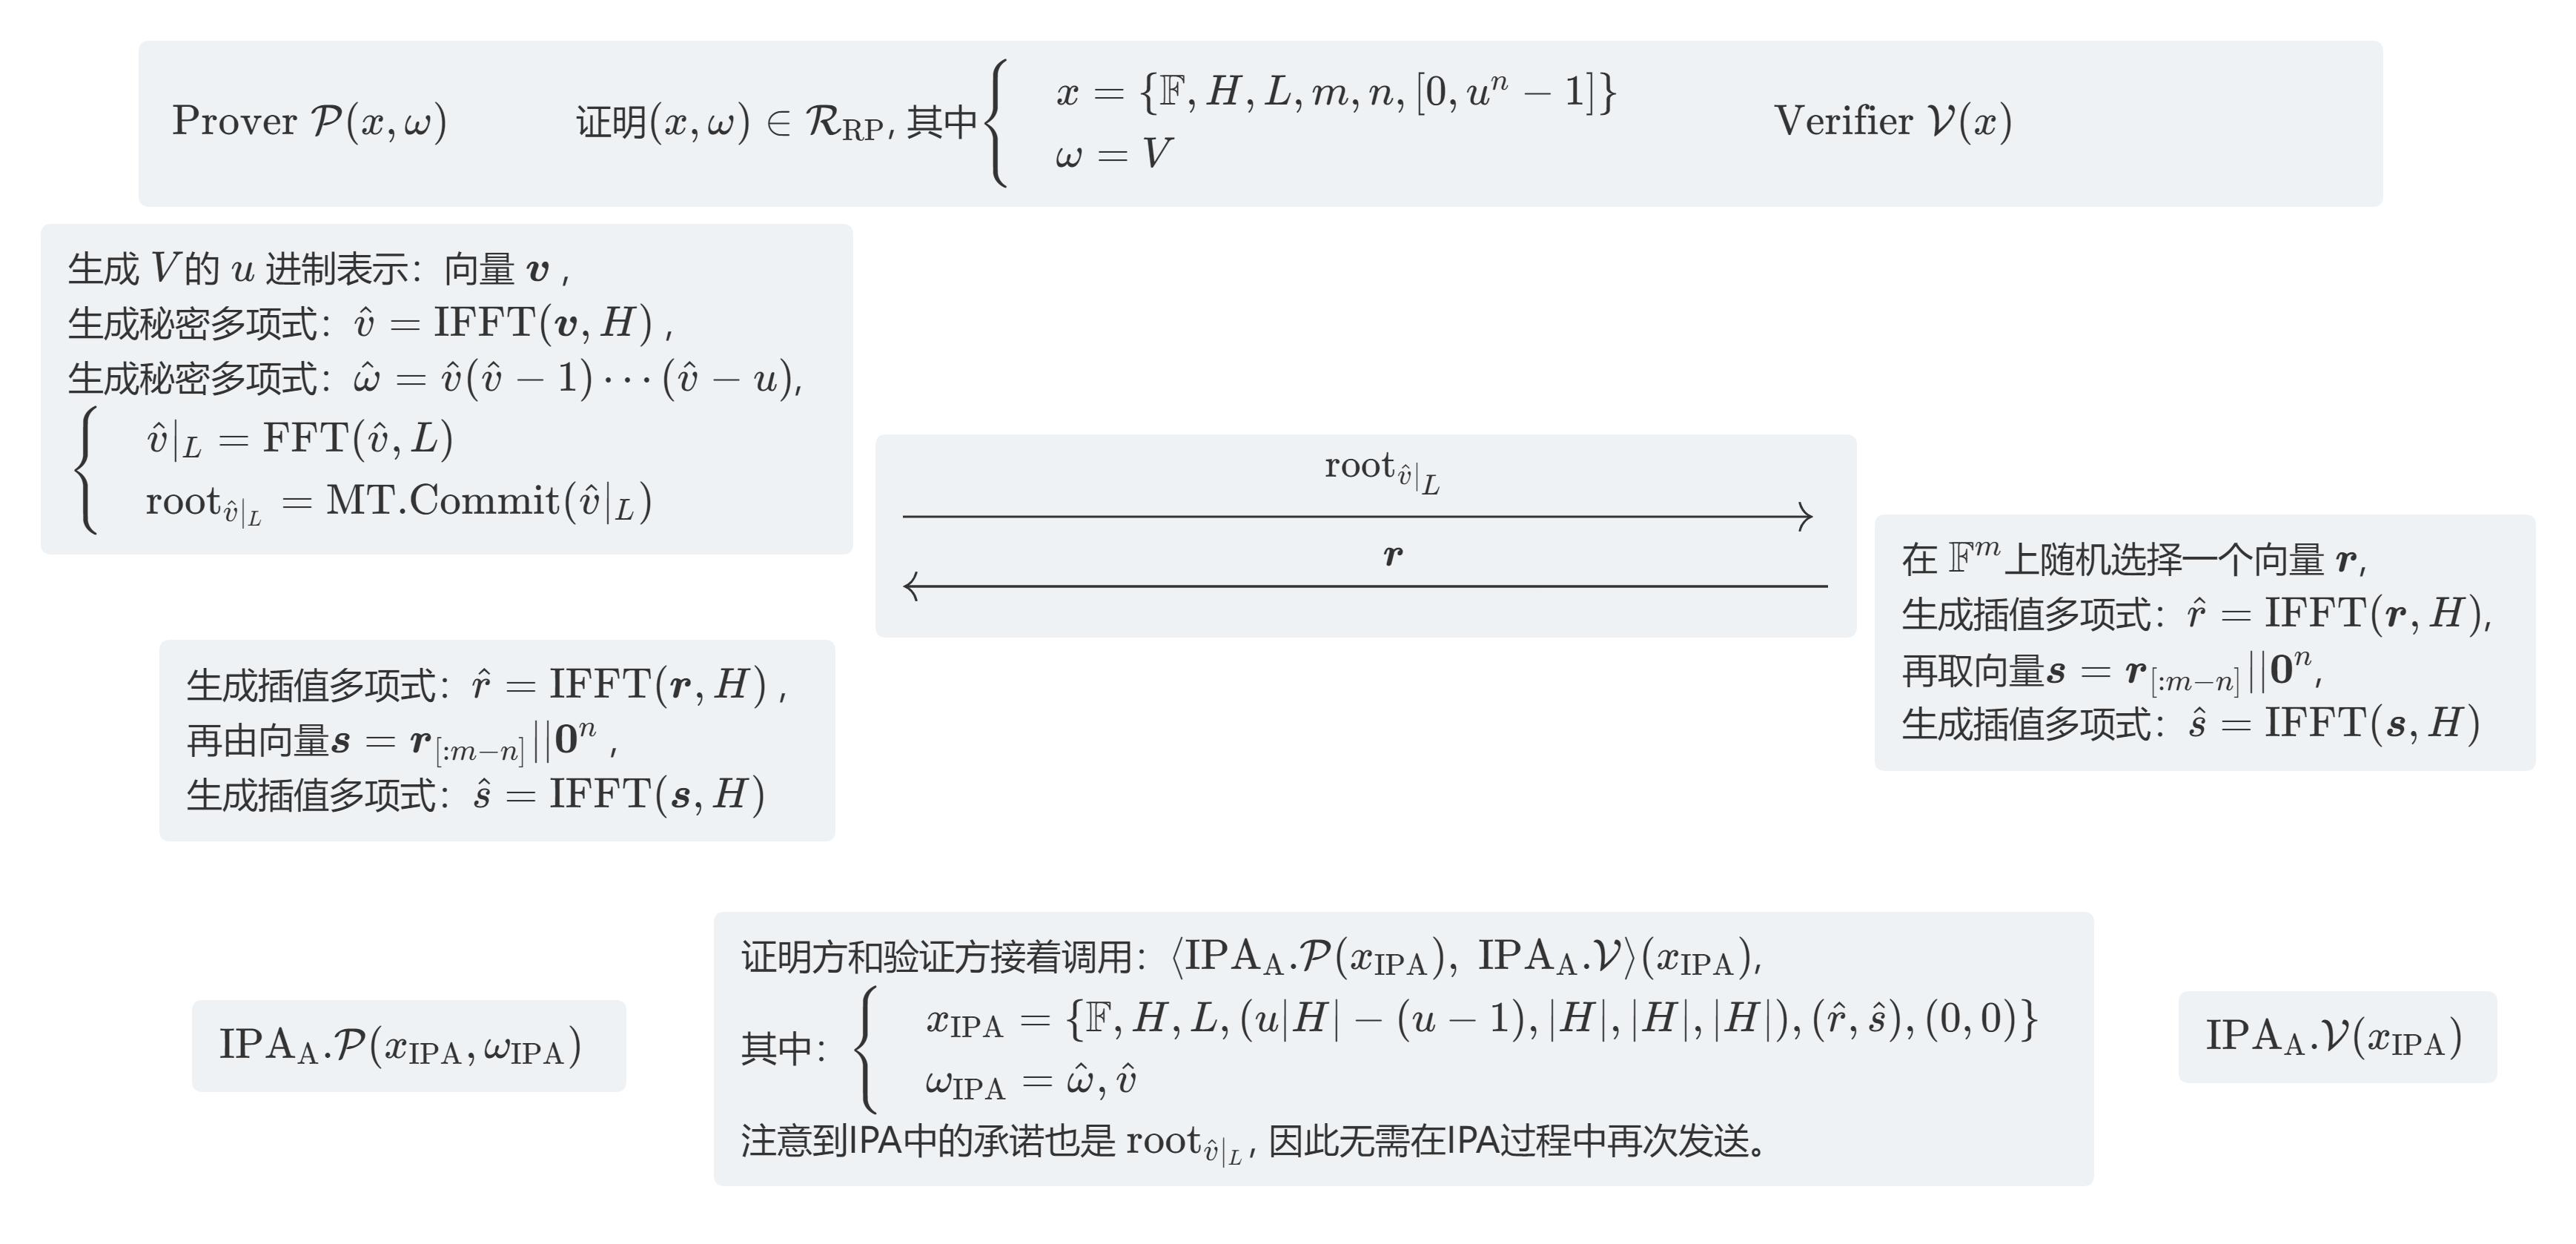
\includegraphics[width=0.85\textwidth]{./include_picture/RP.png}
  \caption{: 范围证明(Range Proof)$\langle \text{RP}.\mathcal{P}(\omega),\text{RP}.\mathcal{V}\rangle(x)$}
  \label{RP流程}
\end{figure}

\subsubsection{批处理范围证明}
基于前述的批处理IPA,我们可以构建一个证明多个秘密值在各自对应范围内的证明。
假设我们要证明秘密值$V_1,...,V_t$分别处于对应范围$[0,u_1^{n_1}-1],...,[0,u_t^{n_t}-1]$,
那么对于任意$j \in \{1,\ldots,t\}$,都有如下公式:
\begin{equation}\begin{aligned}&v_j\odot(v_j-1^m)\odot\cdots\odot(v_j-u_j^m)=0^m,\\&v_j\odot(1^{m-n_j}||0^{n_j})=0^m\end{aligned}\end{equation}\par
其中$m\ge\max\{n_1,...,n_t\}$。进一步转换上述公式,可以推出:对于任意$j \in \{1,\cdots,t\}$,都有如下公式:
\begin{equation}\begin{aligned}
&\langle v_j\odot(v_j-1^m)\odot...\odot(v_j-u_j^m),r\rangle=0,\\
&\langle v_j,(r^{m-n_j}||0^{n_j})\rangle=0\label{第2次调用B-IPA}
\end{aligned}\end{equation}\par
对于公式(\ref{第2次调用B-IPA}),可以利用批处理IPA来证明,即输入设为:
\begin{equation}\begin{aligned}
&x=(\mathbb{F},H,L,\{k_j\}_{j \in [4t]},\{\hat{r}_j\}_{j\in [2t]},\{y_j\}_{j \in [2t]}),\\
&w=\hat{w}_1,...,\hat{w}_t,\hat{v}_1,...,\hat{v}_t,
\end{aligned}\end{equation}\par
其中一些变量满足如下关系:
\begin{equation}\begin{aligned}
&\{k_j\}_{j\in [t]}=\underbrace{u_1|H|-(u_1-1),...,t_t|H|-(u_t-1)}_t,\\
&\{k_j\}_{j\in [t+1,4t]}=\underbrace{|H|,...,|H|}_{3t},\\
&\{\hat{r}_j\}_{j\in [2t]}=\underbrace{\hat{r},...,\hat{r}}_t,\underbrace{\hat{s}_1,...,\hat{s}_t}_t,\\
&\{y_j\}_{j\in [2t]}=\underbrace{0,...,0}_{2t}.
\end{aligned}\end{equation}\par
其中对任意$j\in \{1,\cdots,t\},\hat{s}_j$和$\hat{v}_j$是$r^{m-n_j}||0^{n_j},v_j$的编码多项式,
以及$\hat{w}_j=\hat{v}_j(\hat{v}_j-1)\cdot\cdot\cdot(\hat{v}_j-u_j)$。\par
\subsubsection{对于任意范围的范围证明}
考虑到实际整数范围证明往往是任意整数,我们需要进一步拓宽前述范围证明的通用性。
为了实现这一点,我们需要利用前述的对范围$[0,u^n-1]$的范围证明。
假设要验证秘密值$V\in[A,B-1]$,其中$A,B$均为任意整数。收到Camenisch\cite{twelve}等人的启发,
我们首先将这个问题进行如下转化:
\begin{equation}V-A\in [0,u^n-1]\wedge V-B+u^n\in [0,u^n-1]\end{equation}\par
其中$u^{n-1}<B<u^n$。基于新的公式,我们成功将任意整数范围的证明转化到了
范围$[0,u^n-1]$的证明上,从而我们可以利用前述的对范围$[0,u^n-1]$的范围证明来
实现任意范围的范围证明。\par
在任意范围的证明流程中,验证方不采用基于秘密值$V$的向量$v$的询问,
而是直接让证明方通过IPA证明$V-A=C$和$V-B+u^n=D$。由于此处IPA不止一个,
因此我们可以引入批处理IPA来加快处理过程。实际上,任意范围的范围证明可以
简单看作基于批处理IPA的多个任意基底范围证明的有效融合。
\subsubsection{补充零知识性}
前述的范围证明实际上并不是零知识性的,它存在两个层面的知识泄露:
\begin{itemize}
  \item 问询环节:在验证者打开默克尔树的承诺时,其可见$l$个$\mathbb{V}|_L$的
        估值。而这些估值与秘密向量$\{v_j\}_{1\le j\le t}$相关,因而会泄露
        $\{V_j\}_{1\le j\le t}$的部分信息。
  \item PRI协议环节:在验证方借助$O(\log{|L|})$轮对码字$\hat{v}_1|_L,\cdots,\hat{v}_L|_L$
        的谕示机访问时,验证方可以根据这些已得的信息获取额外的其他信息。
\end{itemize}\par
因此,我们采取与张、谢等人\cite{Fourty-two}相似的处理。\par
对于第一个知识泄露,我们使证明者采取以下措施:
选择一个度为$l$的随机多项式$\hat{\delta}_j$,利用其掩盖$\hat{v}_j$,即
$\hat{v}^{\prime}_j=\hat{v}_j+\hat{Z}_H\cdot\hat{\delta}_j$,其中$\hat{Z}_H$是
陪集$H$上的“消失”多项式,即对$\forall h\in H,\hat{Z}_H(h)=0$.\par
对于第二个知识泄露,我们使证明者采取同样的措施,即使用随机多项式$\hat{\gamma}$来掩盖
秘密多项式$\hat{v}$,并控制$\hat{\gamma}$的度在$(u_{\max}+1)|H|+u_{\max}(l-1)$。
基于以上处理,我们给出批处理的零知识范围证明的流程,如图(\ref{ZKRP流程})所示。
\begin{figure}[H]
  \centering
  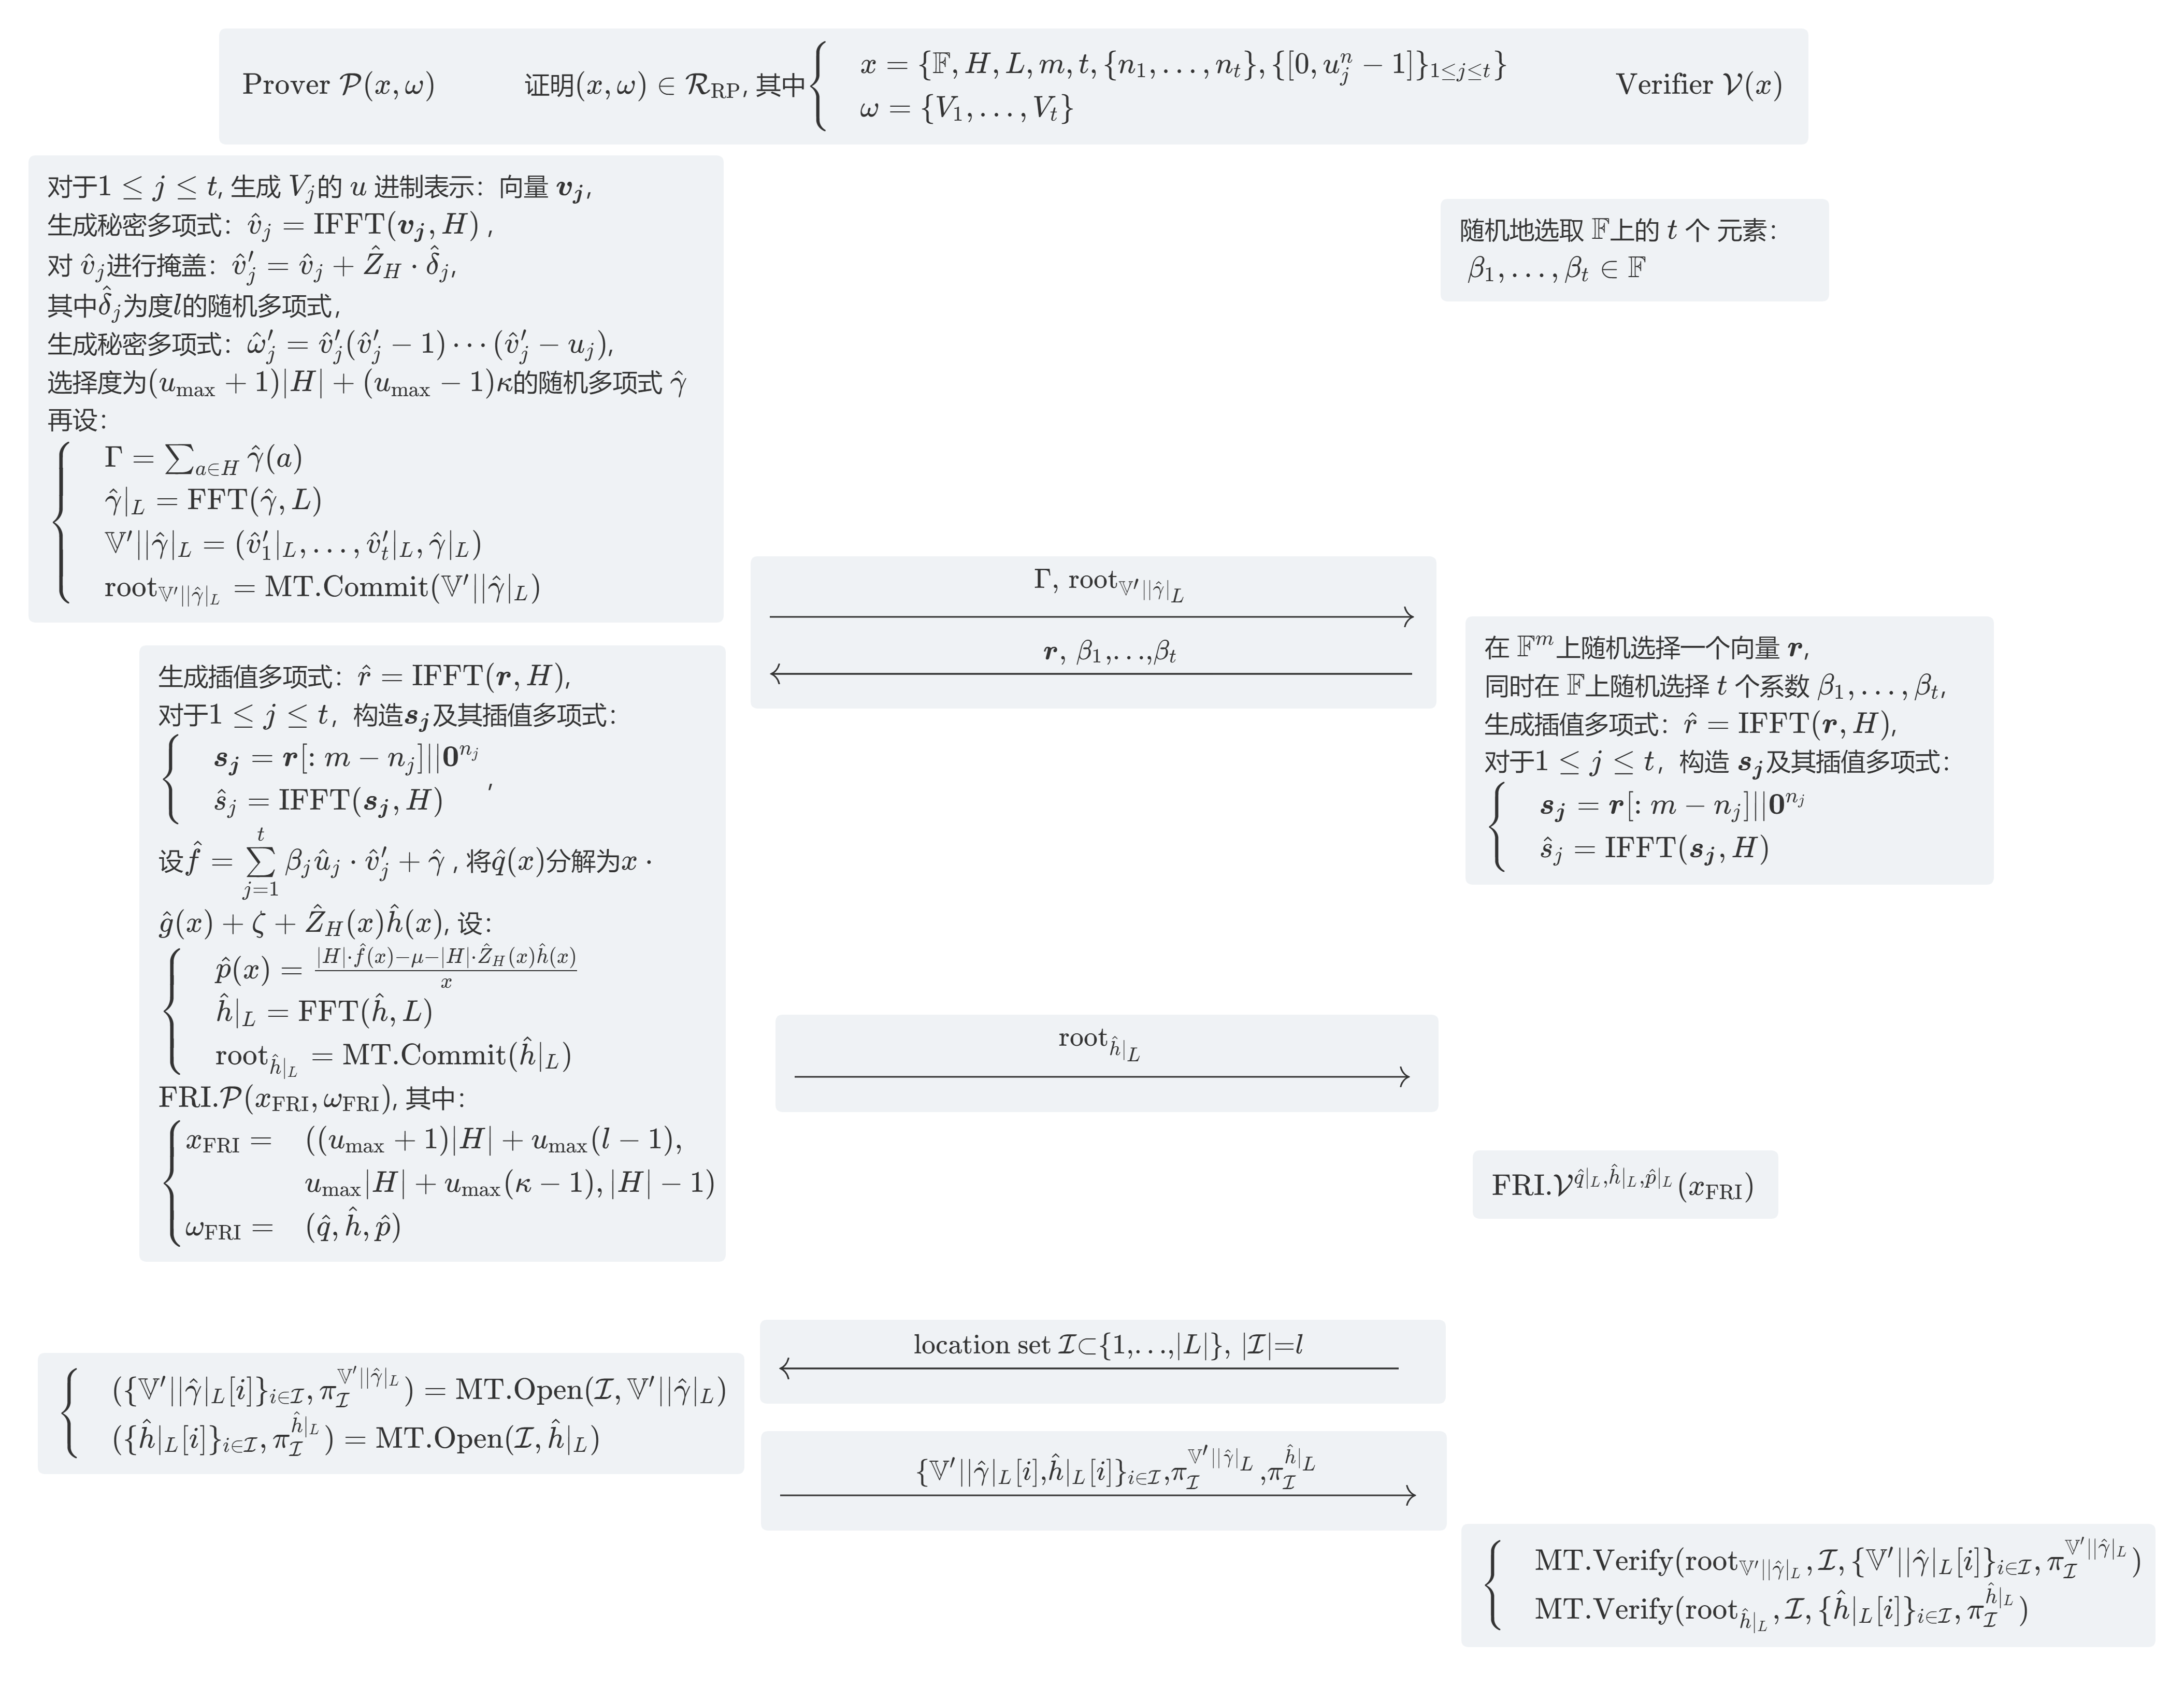
\includegraphics[width=0.85\textwidth]{./include_picture/ZKRP.png}
  \caption{: 零知识范围证明(Zero-Knowledge Range Proof)$\langle \text{RP}_{\text{zk}}.\mathcal{P}(\omega),\text{RP}_{\text{zk}}.\mathcal{V}\rangle(x)$}
  \label{ZKRP流程}
\end{figure}\par
可以证明,以上流程具有完备性(Completeness)、正确性(Soundness)、
知识论证性(Argument of knowledge)、诚实验证者前提的零知识性(Honest-verifier zero knowledge)。


%********************作品成果展示与安全性分析********************
\section{作品成果展示与安全性分析}
\subsection{安全性分析}

%********************前景展望********************
\section{前景展望}

%********************结论********************
\section{结论}

%********************参考文献********************
\section{参考文献}

\begin{thebibliography}{2}
	\bibitem{czh_1.1}Adepu S, Adler R F. A comparison of performance and preference on mobile devices vs. desktop computers[C]//2016 IEEE 7th Annual Ubiquitous Computing, Electronics \& Mobile Communication Conference (UEMCON). IEEE, 2016: 1-7.
	
	\bibitem{czh_1.2}Bettini C. Privacy protection in location-based services: a survey[J]. Handbook of mobile data privacy, 2018: 73-96.
	
	\bibitem{czh_1.3}Liu D, Gao X, Wang H. Location privacy breach: Apps are watching you in background[C]//2017 IEEE 37th international conference on distributed computing systems (ICDCS). IEEE, 2017: 2423-2429.
	
	\bibitem{czh_1.4}Jayaraman P P, Yang X, Yavari A, et al. Privacy preserving Internet of Things: From privacy techniques to a blueprint architecture and efficient implementation[J]. Future Generation Computer Systems, 2017, 76: 540-549.
	
	\bibitem{czh_1.5}Song J H, Wong V W S, Leung V C M. Secure location verification for vehicular ad-hoc networks[C]//IEEE GLOBECOM 2008-2008 IEEE Global Telecommunications Conference. IEEE, 2008: 1-5.
	
	\bibitem{czh_6.1}Gruteser M, Grunwald D. Anonymous usage of location-based services through spatial and temporal cloaking[C]//Proceedings of the 1st international conference on Mobile systems, applications and services. 2003: 31-42.
	
	\bibitem{czh_6.2}李梦涵,钟小宇,李丽红.基于位置服务的隐私保护研究[J].信息与电脑(理论版),2022,34(15):248-250.
	
	\bibitem{czh_6.3}Zhu X, Ayday E, Vitenberg R. A privacy-preserving framework for outsourcing location-based services to the cloud[J]. IEEE Transactions on Dependable and Secure Computing, 2019, 18(1): 384-399.
	
	\bibitem{czh_6.4}Samarati P, Sweeney L. Generalizing data to provide anonymity when disclosing information[C]//PODS. 1998, 98(188): 10-1145.
	
	\bibitem{czh_6.5}Gruteser M, Grunwald D. Anonymous usage of location-based services through spatial and temporal cloaking[C]//Proceedings of the 1st international conference on Mobile systems, applications and services. 2003: 31-42.
	
	\bibitem{czh_6.6}McSherry F, Talwar K. Mechanism design via differential privacy[C]//48th Annual IEEE Symposium on Foundations of Computer Science (FOCS'07). IEEE, 2007: 94-103.
	
	\bibitem{czh_6.7}张琳, 刘彦, 王汝传. 位置大数据服务中立足于差分隐私的数据发布技术[J]. 通信学报,2016, 37(9): 46-54.
	
	\bibitem{czh_6.8}Wei J, Lin Y, Yao X, et al. Differential privacy-based location protection in spatial crowdsourcing[J]. IEEE Transactions on Services Computing, 2019, 15(1): 45-58.
	
	\bibitem{czh_5.1}张梦凡等.《2022中国卫星导航与位置服务产业发展白皮书》发布 北斗进入规模应用发展新阶段  [EB/OL] .光明网.(2022—02—19)[2023—04—09].https://tech.gmw.cn/2022-05/19/content\_35746711.htm
	
	
\end{thebibliography}



% 公式示例展示如下:
% \begin{align}
% \underset{{\bf I}_c \sim \boldsymbol\Im_c}{\mathrm{\text P}}
%  \Big( \mathcal C({\bf I}_c) \neq \mathcal C({\bf I}_c + \boldsymbol \rho) \Big) \geq \delta ~~~\text{s.t.}~~||\boldsymbol\rho||_p \leq \xi,
% \label{eq:def1}
% \end{align}

%********************格式要求********************
\section{——————模板分割线——————}
\section{简介}
\setParDis %设置段间距为 0
\begin{spacing}{1.5}
  第三十三届“冯如杯”主赛道论文一律由在计算机上输入、排版、定稿后转成PDF格式,
在集中申报时通过网络上传。\textbf{论文封面及全文中不能出现作者姓名、学院、专业、指导老
师的相关信息}。包括5个部分, 顺序依次为: \par 
  % 段落间可加入\par进行换行,代替两行回车的写法
  \begin{itemize}
    \item 封面(中文)
    \item 中文摘要、关键词(中文、英文)
    \item 主体部分
    \item 结论
    \item 参考文献
  \end{itemize}

\section{论文的书写规范}

论文正文部分需分章节撰写,每章应另起一行。
章节标题要突出重点,简明扼要、层次清晰。字数一般在15字以内,不得使用标点符号。标题中尽量不采用英文缩写词,对必须采用者,应使用本行业的通用缩写词。  层次以少为宜,根据实际需要选择。三级标题的层次按章(如“一、”)、节(如 “(一)”)、条(如“1.”)的格式编写,各章题序的阿拉伯数字用 Times New Roman 体。  

\subsection{字体和字号}
论文题目:二号,华文中宋体加粗,居中。

副标题:三号,华文新魏,居右(可省略)。

章标题:三号,黑体,居中。

节标题:四号,黑体,居左。

条标题:小四号,黑体,居左。

正文:小四号,中文字体为宋体,西文字体为Times New Roman体,首行缩进,两端对齐。

页码:五号Times New Roman 体,数字和字母\par

\subsection{页边距及行距}
学术论文的上边距:25mm;下边距:25mm;左边距:30mm;右边距 20mm。
章、节、条三级标题为单倍行距,段前、段后各设为0.5行(即前后各空0.5行)。
正文为 1.5 倍行距,段前、段后无空行(即空0行)。

\subsection{页眉}
页眉内容为北京航空航天大学第三十三届“冯如杯”竞赛主赛道参赛作品,内容居中。
页眉用小五号宋体字,页眉标注从论文主体部分开始(引言或第一章)。
请注意论文封面无页眉。

\subsection{页码}
论文页码从“主体部分(引言、正文、结论)”开始,直至“参考文献”结束,用五号阿
拉伯数字连续编码,页码位于页脚居中。\textbf{封面、题名页不编页码。}

摘要、目录、图标清单、主要符号表用五号小罗马数字连续编码,页码位于页脚居中。

\subsection{图、表及其附注}
图和表应安排在正文中第1次提及该图、表的文字的下方,当图或表不能安排在该页时,
应安排在该页的下一页。

\subsubsection{图}
图题应明确简短,\textbf{用五号宋体加粗},数字和字母为\textbf{五号Times New Roman体
加粗},图的编号与图题之间应空半角2格。图的编号与图题应置于图下方的居中位置。图内文字
为\textbf{5号宋体},数字和字母为\textbf{5号Times New Roman体}。曲线图的纵横坐标必
须标注“量、标准规定符号、单位”,此三者只有在不必要注明(如无量刚等)的情况下方可省略。
坐标上标注的量的符号和缩略词必须与正文中一致。

\subsubsection{表}
表的标号应采用从1开始的阿拉伯数字编号,如:“表 1”、“表 2”、……。表编号应一直连续到附录
之前,并与章、节和图的编号无关。只有一幅表,仍应标为“表 1”。表题应明确简短,用\textbf{五号宋体
加粗},数字和字母为\textbf{五号Times New Roman体加粗},表的编号与表题之间应空半角2格。表的编号与
表头应置于表上方的居中位置。表内文字为\textbf{5号宋体},数字和字母为\textbf{5号Times New Roman体}。  

\subsubsection{附注}
图、表中若有附注时,附注各项的序号一律用“附注+阿拉伯数字+冒号”,如:“附注1:”。

附注写在图、表的下方,一般采用5号宋体。

\subsubsection{参考文献}
凡有直接引用他人成果(文字、数字、事实以及转述他人的观点)之处,均应加标注说明列于参考文献中,
以避免论文抄袭现象的发生。

标注格式:引用参考文献标注方式应全文统一,标注的格式为[序号],放在引文或转述观点的最后
一个句号之前,所引文献序号用小4号Times New Roman体、以上角标形式置于方括号中,如“……成果”$^{[1]}$。
\section{图表模板}
图表示例展示如下:

%插入一张图片
\begin{figure}[H] %H为当前位置,!htb为忽略美学标准,htbp为浮动图形
    \centering %图片居中
    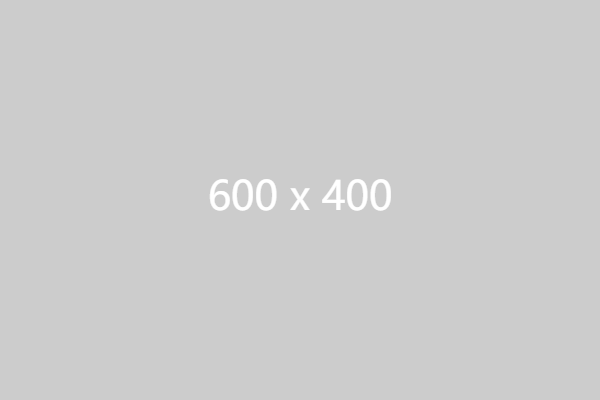
\includegraphics[width=0.8\textwidth]{example-image-2.png} %插入图片,[]中设置图片大小,{}中是图片文件名
    \caption{example\_caption} %最终文档中希望显示的图片标题
    \label{example_label} %用于文内引用的标签
\end{figure}

% 一行三张子图并排示意
\begin{figure}[htbp]
  \begin{subfigure}{0.31\textwidth}
    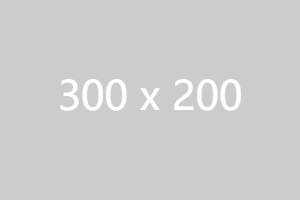
\includegraphics[width=\linewidth]{example-image-1.png}
    \caption{示意图1} \label{fig:9aaa}
  \end{subfigure}%
  \hspace*{\fill}   % maximize separation between subfigures
  \begin{subfigure}{0.31\textwidth}
    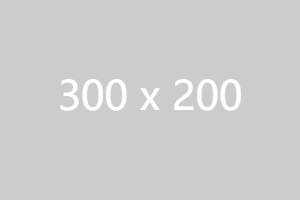
\includegraphics[width=\linewidth]{example-image-1.png}
    \caption{示意图2} \label{fig:9bbb}
  \end{subfigure}
  \hspace*{\fill}   % maximizeseparation between subfigures
  \begin{subfigure}{0.31\textwidth}
    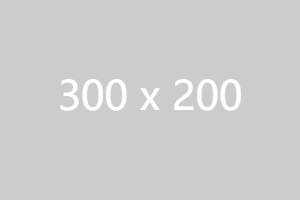
\includegraphics[width=\linewidth]{example-image-1.png}
    \caption{示意图3} \label{fig:9ccc}
    \end{subfigure}
\caption{一行三张子图并排示意}
\label{qmix-train}
\end{figure}


% 2*2四张子图示意
\begin{figure}[htbp]
  \begin{subfigure}{0.48\textwidth}
    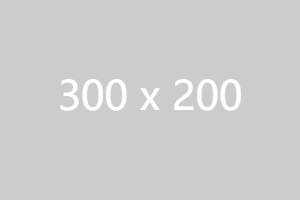
\includegraphics[width=\linewidth]{example-image-1.png}
    \caption{示意图1} \label{fig:8a}
  \end{subfigure}%
  \hspace*{\fill}   % maximize separation between subfigures
  \begin{subfigure}{0.48\textwidth}
    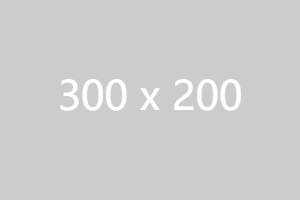
\includegraphics[width=\linewidth]{example-image-1.png}
    \caption{示意图2} \label{fig:8b}
  \end{subfigure}\\
  %\hspace*{\fill}   % maximizeseparation between subfigures
  \begin{subfigure}{0.48\textwidth}
    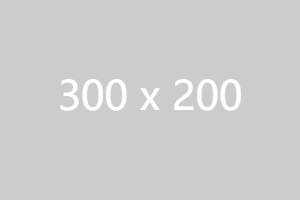
\includegraphics[width=\linewidth]{example-image-1.png}
    \caption{示意图3} \label{fig:8c}
  \end{subfigure}
  \hspace*{\fill}   % maximize separation between subfigures
  \begin{subfigure}{0.48\textwidth}
    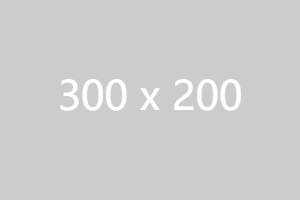
\includegraphics[width=\linewidth]{example-image-1.png}
    \caption{示意图4} \label{fig:8d}
  \end{subfigure}
\caption{2*2四张子图示意} \label{fig:8}
\end{figure}

%插入一个表格

\begin{table*}[H]
\centering
\caption{表格使用示例}
\begin{tabular}{|l||c|c|c|c|c|c|}
\hline
{\textbf{表头 1}}     &  表头 2 	    & 表头 3 	  & 表头 4     & 表头 5 		\\ \hline\hline
内容 11 		          & 内容 12				& 内容 13		& 内容 14 	 & 内容 15		\\ \hline
内容 21	              & 内容 22				& 内容 23		& 内容 24	   & 内容 25		\\ \hline


\end{tabular}
\end{table*}


%再插入另一种表格
\begin{table}[H]
\caption{三线表使用示例}
\centering
\begin{tabular}{ccccc}
\hline  
\textbf{方法} & \textbf{表头 1} & \textbf{表头 2} & \textbf{表头 3} & \textbf{表头 4} \\ 
\hline  
方法1 & 数据  & 数据  & 数据  & 数据\\
方法2 & 数据  & 数据  & 数据  & 数据\\
\hline
\end{tabular} 
\end{table} 

\section*{结论}% section*生成无标号章节
\addcontentsline{toc}{section}{结论} % 将无标号章节添加至目录
论文的结论单独作为一章,但不加章号。

注意: 文件大小不超过5M。

\end{spacing}

\newpage

% XSP 2023/3/16: bib支持不全,暂时改为手动
% \section*{参考文献} % section*生成无标号章节题目
% \addcontentsline{toc}{section}{参考文献} % 将无标号章节添加至目录
% % 著作: [序号]作者.书名[标识码].出版地:出版社,出版年.
% [1]张志建.严复思想研究[M].桂林:广西师范大学出版社,1989. 

% % 译著: [序号]国名或地区(用圆括号)原作者.书名[标识码].译者.出版地:出版社,出版年.
% [2](英)霭理士.性心理学[M].潘光旦译.北京:商务印书馆,1997.

% % 古典文献 文史古籍类引文后加序号,再加圆括号,内加注书名、篇名

% % 论文集: [序号]编者.书名[标识码].出版地:出版社,出版年.
% [3]伍蠡甫.西方论文选(下册)[C].上海:上海译文出版社,1979.

% % 期刊文章: [序号]作者.篇名[标识码].刊名,年,(期).
% [4]叶朗.《红楼梦》的意蕴[J].北京大学学报(哲学社会科学版),1989,(2)

% % 报纸文章: [序号]作者.篇名[标识码].报纸名,出版日期(版次)
% [5]谢希德.创造学习的新思路[N].人民日报,1998-12-25(10)

% % 外文文献: 要求外文文献所表达的信息和中文文献一样多,但文献类型标识码可以不标出。
% [6]Mansfeld, R.S. \& Busse. \textit{T.V. The Psychology of creativity and discovery}, Chinago:
% NelsonHall, 1981




% \begingroup
% \setstretch{2.0}    %行距2
% \setlength{\bibsep}{0pt}    %段前段后0
% \begin{adjustwidth}{0.42cm}{0.42cm} %左右缩进0.42cm
% \bibliography{references}
% \end{adjustwidth}
% \endgroup


\bibliography{references}


\end{document}
